\documentclass[UTF-8,a4paper,zihao=-4]{ctexart}
\usepackage[a4paper,left=3cm,right=2.5cm,top=3cm,bottom=2.5cm]{geometry}
\usepackage{graphicx} % Required for inserting images
\usepackage[backend=biber,style=gb7714-2015]{biblatex} 
\usepackage[labelfont=bf,textfont=bf]{caption}
\addbibresource{ref.bib} %待补上参考文献 
\usepackage{amsmath,amssymb}   % 公式
\usepackage{graphicx}          % 插图
\usepackage{booktabs}           % 三线表
\usepackage{hyperref}           % 超链接（最后加载，少数例外）
\usepackage{placeins}
\usepackage{subcaption}
\usepackage{csvsimple}
\usepackage{listings}
\usepackage{xcolor}
\usepackage{float}
\pagestyle{plain} 
\ctexset{
  section = {
    number = \chinese{section},   % 中文数字：一、二、三…
    format = \zihao{3}\heiti\centering,
    aftername = \quad,            % 编号和标题之间的空格（可调）
    % 如果你想变成“一、绪论”（带顿号），把 aftername 改成 \hspace{1em} 或直接写顿号
  }
}
\makeatletter
\renewcommand{\maketitle}{
    \begin{center}
        \vspace*{-2cm}
        {\zihao{2}\heiti\@title\par}
    \end{center}
}
\makeatother

\makeatletter
\renewenvironment{abstract}
{
    \begin{center}
        {\zihao{-3}\textbf{摘要}}
    \end{center}
    \zihao{-4}
}
{}
\makeatother

\lstset{
    language=Python,
    basicstyle=\ttfamily\small,
    numbers=left,
    numberstyle=\tiny,
    frame=single,
    breaklines=true,
    columns=fullflexible
}

\begin{document}

\title{海上人员运载方案的高效率编排}
\date{}
\maketitle


%%%%%摘要%%%%%
\begin{abstract}

\textbf{针对问题一：} 本文首先将单架直升机从陆地机场出发、依次访问若干海上设施并返回原机场的完整运输过程定义为一个架次，在此基础上建立考虑异构机型、座位容量、最多 5 次海上着陆及途中可选加油的单向出海运输模型。对于起点为 LAND 的人员，将实际起飞机场作为待确定变量，并结合固定机场人员统一进行架次划分；以总飞机使用时间为首要目标，并依次考虑人员总在途时间、燃油消耗和座位利用率，建立\textbf{严格字典序优化模型}。求解时先利用\textbf{动态规划}完成同一目的地人员的机场分配和分批运输，再采用\textbf{节约合并和多尺度大邻域搜索}对已有架次进行\textbf{重组}，同时将搜索得到的可行路线加入路线池，并通过受限集合划分对候选架次进行重新组合。最终完成 1600 名人员的出海运输，\textbf{共安排 92 个架次，总飞机使用时间为 14991 分钟，人员总在途时间为 116061 分钟，总燃油消耗量为 120437.70 kg，座位利用率为 48.5224\%。}
    
\textbf{针对问题二：} 本文将出海、海返与设施间穿梭需求统一表示为带取送先后关系的人员运输需求，建立异构机型、动态载客量、最多5次海上着陆及途中可选加油约束下的路线集合划分模型。先按起终点聚合需求并\textbf{构造单类可行架次}，再以节约合并产生初始联合运输方案；随后\textbf{利用合并、转移、交换、二路线重分配和三路线压缩}等大邻域算子\textbf{扩充路线池}，并通过\textbf{整数规划}进行全局重组。目标采用严格字典序，依次最小化总飞机使用时间、人员总在途时间和总燃油消耗量，在前三层目标不变时最大化座位利用率。最终为4000名人员\textbf{安排118个架次，总飞机使用时间为20751分钟，人员总在途时间为248493分钟，总燃油消耗量为161473.10 kg，座位利用率为76.8449\%}
    
\textbf{针对问题三：}本文在前述问题的取送模型基础上，引入\textbf{时间窗}构造机队排队模型，按照人员起终点、时间兼容关系和燃油量等约束构造基础运输批次形成初始路线池，随后通过\textbf{路线合并、人员重分配和临时人员插入}扩充路线池，统一完成架次选择、具体飞机分配和起飞时刻安排。对于两个求解阶段，第一阶段以总飞机使用时间为首要目标进行严格字典序优化，得到非临时任务的飞机使用时间基准；第二阶段在不超过该基准的条件下，优先最大化临时人员完成数量，再依次优化总飞机使用时间、人员总在途时间、总架次数、燃油消耗量和座位利用率。最终完成全部3840名非临时人员和\textbf{154名临时人员的运输，共安排164个架次，总飞机使用时间为32887分钟，人员总在途时间为269475分钟，总燃油消耗量为247971.70千克，座位利用率为54.6549\%。}

\noindent \textbf{关键词：}直升机运载计划；取送问题；集合划分；字典序优化；大邻域搜索；CP

\end{abstract}

%%%%%问题重述%%%%%
\newpage
\section{问题背景与重述}
\subsection{问题背景}

海上油田由陆地机场、海上油气田及配套生产设施共同构成。为保证油气开采、设备检维修和生产保障等工作连续开展，各类人员需要长期驻守海上设施，并按照任务安排完成出海、海返或不同设施之间的穿梭。海上设施距离陆地较远，人员运输主要依靠直升机完成，因而运载计划不仅关系到人员能否按要求到达，也直接影响飞机使用时间、燃油消耗和整体运输效率。

本题所研究的运输网络包括3座陆地机场和52座海上设施，其中8座设施可以为直升机加油。每个架次均从某一机场起飞，连续停靠若干海上设施后返回原机场，途中最多进行5次海上着陆；人员必须由同一架次送达，不得换乘。不同机型在座位数、飞行速度、单位距离油耗、油箱容量和最低安全余油量等方面存在差异，而同一架次又可能同时承担人员送出、接回和设施间转运任务。因此，我们需要在满足取送顺序、航段容量、燃油安全和运行时间等约束的基础上，对人员分组、机型选择、停靠顺序及加油安排进行统一编排，并以总飞机使用时间为主要指标评价运载方案，具体表现为以下三个问题：

\subsection{问题要求}

\begin{enumerate}
    \item \textbf{单向出海运输计划}

    本问需要考虑安排1600名人员从陆地机场前往海上设施的运输需求，无需考虑最早可登机时间、最晚需到达时间和业务性质优先级，同时本问假设可用飞机数量充足。本问目标是为全部人员确定所乘机型、架次、实际起飞机场和海上停靠顺序，在满足座位容量、最多5次海上着陆、燃油消耗及最低安全余油等约束的前提下，优先减小总飞机使用时间，并在该目标基础上进一步优化人员总在途时间、燃油消耗和座位利用率，最终需要给出人员安排表和架次路线表，并统计总飞机使用时间、人员总在途时间、总架次数、总燃油消耗量及座位利用率。

    \item \textbf{出海、海返与穿梭联合运输计划}

    本问继承问题一发展而来，在人数上扩大为4000人员的运输需求；在运输上，运输航程扩展为出海、海返、穿梭三种，由此需要进一步确定海返与穿梭人员在同一架次中的上下机位置，使每名人员的上机位置早于下机位置，并在上机后第一次到达终点时下机，同时满足各航段实际载客量均不得超过机型座位数的限制。在满足取送先后、起降机场一致、着陆次数、燃油和安全余油约束的条件下，本问要求对三类需求进行联合编排，仍以总飞机使用时间最小为首要目标，并尽可能优化人员在途时间、燃油消耗和座位利用率，最终按照指定格式给出4000名人员的安排和全部架次路线，并计算相应评价指标。

    \item \textbf{带时间要求和机队限制的多日排班}

    本问在问题二需求的基础上增加了最早离开起点时刻、最晚送达时刻和业务性质，规划区间为2026年8月3日00:00至8月10日00:00。与此同时，本问要求只能使用题目给出的24架直升机，每架飞机在规划开始时停放于所属机场；飞机须在每日06:00至18:00之间起飞，不晚于20:00返回机场，且两个相邻架次之间至少保留30分钟机场周转时间。

    四类任务按照应急处置、增储上产、常规倒班和临时任务的次序进行保障，其中临时任务允许取消。需要先排除临时任务，为其余人员编排可行计划并得到基准总飞机使用时间；再以该时间为上限加入临时人员，优先使得到满足的临时运输人数尽可能多，并在此基础上继续优化总飞机使用时间、人员总在途时间、架次数、燃油消耗和座位利用率，最终给出具体飞机的多日路线与人员安排，并说明临时任务满足情况及各项评价指标。
\end{enumerate}


%%%%%问题分析%%%%%
\section{问题分析}
\subsection{问题一分析}
问题一主要考虑 1600 名人员从陆地机场前往各海上设施的出海运输。由于本问中人员只需要从机场前往自己的目的设施，所以对于同一个架次，所有人员在机场上机后会随着飞机到达不同设施依次下机，机上的人数不会在途中增加。因此在人员容量方面，只需要先保证一个架次起飞时的人数不超过对应机型的座位数，再安排不同目的设施的停靠顺序。

对于起飞机场，题目中一部分人员已经指定了具体机场，这部分人员只能由对应机场出发；而标记为 LAND 的人员没有指定具体机场，因此还需要根据实际运输路线在 A01、A02 和 A03 中选择起飞机场。同时，三种机型的座位数、速度和燃油参数都不同，而不同的设施访问顺序也会影响一个架次的总飞行时间、人员在途时间和燃油消耗。所以我们在安排一个架次时，需要同时考虑人员组合、起飞机场、机型、设施停靠顺序以及是否需要途中加油。

由于人员数量较多，如果直接对所有人员组合进行枚举，再分别计算不同机场、机型和设施顺序，计算量会很大。因此我们先按照人员的目的设施进行分组，对同一目的地的人员先完成机场分配和架次划分，得到一个完整的初始运输方案。之后再尝试把不同架次进行合并和重新组合，如果新的组合能够减少飞机使用时间，则保留这种方案；同时将搜索过程中得到的可行架次记录下来，再从这些候选架次中重新选择整体组合。通过这样的方式逐步缩小总飞机使用时间，并在总飞机使用时间不变的情况下继续比较人员在途时间、燃油消耗和座位利用率。

\subsection{问题二分析}
问题二在问题一单向出海运输的基础上加入海返与设施间穿梭需求。此时，一名人员在某一航段是否占用座位，不再只由其目的地决定，而是同时取决于上机位置、下机位置和停靠顺序。特别地，同一设施停靠时执行“先下后上”，释放的座位能够继续承担后续航段的运输任务。因此我们可以得到：单架次累计运输人数可以超过该机型座位数，但任一航段的机上人数均不能超过容量。

穿梭需求还引入了有向的取送先后约束。若一个架次同时承担 $F_i\to F_j$ 与 $F_j\to F_i$ 的需求，则简单的不重复停靠序列可能无法满足全部先后关系，需要允许在5次海上着陆范围内重复停靠部分设施。与此同时，显式机场需求必须从指定机场起降，而起点或终点为 LAND 的人员可以随架次绑定到任一陆地机场。由此，问题二可以视为带异构机型、动态容量、取送先后和可选加油的开放路线生成问题；由于每个架次最终必须返回出发机场，在组合层面又构成一个整数集合划分问题。

求解时若直接枚举4000名人员的分组、停靠顺序、机型和加油决策，会导致求解空间巨大难以计算，考虑到问题二没有个人时间窗与飞机数量限制，同一起终点的人员在可行性和目标贡献上具有同质性，故我们先将人员聚合为264个有向 OD 类，在聚合层面生成架次模板，再利用自适应大邻域搜索扩充高质量路线池，最后由整数主问题对候选路线进行全局重组。该方法避免了仅依靠局部合并确定最终方案，同时还保留了对每条路线取送顺序、燃油和动态容量的逐航段检验。


\subsection{问题三分析}
问题三在问题二海上联合运输问题的基础上，进一步增加了人员时间窗、业务类型、具体飞机数量和规划周期等约束。因此方案的可行性不仅由人员起终点和设施访问顺序决定，还同时受到架次执行日期、时刻以及同一飞机前后的任务衔接关系影响。所以我们认为问题三可以归为带时间窗的取送路径优化与有限机队排班相耦合的问题。

对于每个人员 $i$，在设计方案时，需要考虑满足取送先后关系，时间的约束。而同一空间路线能否执行，则取决于是否存在一个同时满足全部乘客时间窗、机场开放时间和当天返场要求的起飞时刻。所以该问题不能只按照起点与终点对人员进行聚合，要在利用OD结构降低停靠顺序搜索规模的基础上对每个候选架次均保存具体的人员编号，并逐人检查时间窗，避免因过度聚合而产生时间上不可执行的方案。另外，题目给定的飞机均有固定的所属机场与机型。同一飞机在任意时刻只能执行一个架次，且返回机场后存在周转时间。因此考虑将机队排班按照机场与机型的配对来划分兼容飞机组，再对每架具体飞机设置互不重叠的时间占用区间。

对于两阶段的决策结构。由于第一阶段不考虑临时人员，只安排应急取送、生产倒班和常规倒班三类必需任务，可以在满足全部硬约束的前提下最小化总飞机使用时间，得到基准值 $B$。第二阶段加入临时任务后，在总飞机使用时间不超过 $B$的前提下，可以选择通过尽量利用既有架次的空余座位来分配临时人员，或通过重新组合必需任务路线释放飞机时间。

为控制因素进一步增加带来的组合规模增大，本文复用了问题二的单架次空间取送、动态容量、燃油与加油可行性部分。先用CP-SAT方法由单架次生成器完成空间路径、取送关系、动态容量、燃油和时间窗检查，将合法架次作为列加入路线池；再根据主问题从路线池中选择架次，并统一分配具体飞机和起飞时刻；最后围绕当前排班，用时间相关大邻域进行路线合并、重分配和临时任务插入，持续生成新的候选列扩充路线池。该方法将复杂的单架次可行性判断与全局机队排班相分离，同时保留二者之间的迭代反馈。

%%%%%准备工作%%%%%
\section{初步准备}
\subsection{模型假设}
\begin{enumerate}
    \item 严格采用附件给出的地点间距离、机型速度、座位数、单位距离油耗、油箱容量和最低安全余油量；飞行速度与单位距离油耗不随载客量变化。
    \item 问题二不考虑最早登机时间、最晚到达时间和业务优先级，也不限制可用飞机数量，因而各架次之间不存在具体飞机衔接与机场周转约束。
    \item 机场、海上设施和加油站不存在并发容量限制；同一架次从某一机场起飞并返回该机场，人员全程不换乘。
    \item 不加油停靠取题设允许的最短时间10分钟，加油停靠取20分钟。由于本问不存在时间窗或同步约束，额外等待只会增加飞机使用时间和人员在途时间，不可能改善字典序目标。
    \item 对起终点相同的人员进行聚合。由于问题二中同一 OD 类人员没有个体差异，聚合不会改变路线可行域；求解完成后再按人员编号还原到具体架次。
\end{enumerate}

%%表%%
\subsection{符号说明}
本文所使用的符号及说明如下表所示。
\begin{table}[htbp]
\centering
\zihao{5}

\caption{符号说明}
\begin{tabular}{ccc}
\toprule
符号 & 说明 & 单位 \\
\midrule
$G$ & 有向 OD 需求类别集合 & -- \\
$\mathcal R$ & 已生成的可行架次模板集合 & -- \\
$n_g$ & OD 类 $g$ 的待运人数 & 人 \\
$x_r$ & 架次模板 $r$ 的采用次数 & 次 \\
$q_{rg}$ & 模板 $r$ 运送 OD 类 $g$ 的人数 & 人 \\
$m_r$ & 模板 $r$ 的海上着陆次数 & 次 \\
$p_{rg},d_{rg}$ & OD 类 $g$ 在模板 $r$ 中的上下机序号 & -- \\
$Q_k$ & 机型 $k$ 的座位数 & 人 \\
$C_k,R_k$ & 机型 $k$ 的油箱容量与最低安全余油量 & kg \\
$b_k,v_k$ & 机型 $k$ 的单位距离油耗与速度 & kg/km, km/h \\
$T_r$ & 模板 $r$ 的飞机使用时间 & min \\
$H_r$ & 模板 $r$ 的人员总在途时间 & min \\
$B_r$ & 模板 $r$ 的燃油消耗量 & kg \\
$P_r,A_r$ & 模板 $r$ 的客座公里与可用座公里 & 人$\cdot$km \\
$\eta$ & 全部架次的座位利用率 & \% \\
\bottomrule
\end{tabular}

\vspace{0.5em}
\parbox{0.9\textwidth}{
\zihao{5}
注：其他符号已在相应部分中说明。
}
\end{table}
\FloatBarrier

%%%%%模型建立与求解%%%%%
\section{模型建立与求解}
\subsection{问题一的模型建立与求解}
\subsubsection{模型的建立}
针对问题一的问题，我们先定义一架飞机从机场出发，访问若干海上设施后返回机场为一个架次，
设某架次为
\begin{equation}
 r=\left(a_r,k_r,S_r,R_r,p_r\right),
\end{equation}
其中 $a_r$ 为起降机场，$k_r\in\{T1,T2,T3\}$ 为机型，$S_r=(s_a,s_b,s_c,\ldots s_m)$为海上设施访问训练，$R_r$为各停靠位置是否加油，$p_r$为该架次负责运输的人员集合。

对每个架次r，我们设设节点 i 到节点 j 的距离为：$d_{ij}$，机型 k 的速度为：$v_k$，于是我们可以得到在这两个节点之间该架次的飞行时间为\begin{equation}t_{ij}^{k_r}=\lceil\frac{60d_{ij}}{v_k}\rceil\end{equation}
于是我们就可以得出该架次总的飞行时间为
\begin{equation}
t_r
=
\sum_{(i,j)\in E_r} t_{ij}^{k_r}
+
\sum_{s\in S_r} \tau_s ,
\end{equation}
其中$E_r$表示第 r 个架次中所有实际飞行航段组成的集合，$\tau_s$表示在海上设施s的停靠时间
\begin{equation}
\tau_s=
\begin{cases}
10, & \text{若设施 $s$ 仅进行人员上下机},\\
20, & \text{若设施 $s$ 同时进行加油作业}.
\end{cases}
\end{equation}
对于人员在途时间，我们设$d_p$表示人员p的目的设施，由于问题一中所有乘机人员都是从机场起飞开始乘坐，所以其在途时间就是$I_p$=从飞机起飞到到达$d_p$的时间，于是人员在途时间就变为了
\begin{equation}
    I=\sum_{p}I_p
\end{equation}
对于燃油要求，我们假设从节点i到节点j，在i时燃油量为$f_i$，从i到j需要消耗燃油两为$f_{ij}$，那么燃油量需要在途径的节点中任意的节点组合（i，j）满足$f_i-f_{ij}\geq$安全余油，否则需要在途中加油。

对于座位利用率，设航段 $(i,j)$ 上的实际载客人数为 $L_{ij}$，
第 $r$ 个架次所采用机型的座位容量为 $C_{k_r}$，
航段 $(i,j)$ 的飞行距离为 $d_{ij}$。
则第 $r$ 个架次的客公里可表示为
\begin{equation}
P_r
=
\sum_{(i,j)\in E_r}
L_{ij}d_{ij},
\end{equation}
其中，$E_r$ 表示第 $r$ 个架次所经过的全部飞行航段集合。

相应地，第 $r$ 个架次的可用座位公里为
\begin{equation}
A_r
=
\sum_{(i,j)\in E_r}
C_{k_r}d_{ij}.
\end{equation}

对于整个运输方案，设候选架次集合为 $\mathcal{R}$，
则总客公里和总可用座位公里分别为
\begin{equation}
P
=
\sum_{r\in\mathcal{R}} P_r,
\end{equation}

\begin{equation}
A
=
\sum_{r\in\mathcal{R}} A_r.
\end{equation}

因此，座位利用率定义为
\begin{equation}
\eta
=
\frac{P}{A}
=
\frac{
\displaystyle
\sum_{r\in\mathcal{R}}
\sum_{(i,j)\in E_r}
L_{ij}d_{ij}
}{
\displaystyle
\sum_{r\in\mathcal{R}}
\sum_{(i,j)\in E_r}
C_{k_r}d_{ij}
}.
\end{equation}

于是一个架次r又可以进一步表示为
\begin{equation}
    r=(q_r,t_r,I_r,F_r,P,A)
\end{equation}
其中$q_r$表示该架次的运输任务和承载人员

$t_r$表示该架次的飞行时间

$I_r$表示该架次的人员在途时间

$F_r$表示该架次的燃油使用情况

$P$表示该架次的载客总公里

$A$表示该架次的可用座位总公里

对于每个架次r我们按照题目要求的在最小化总飞机使用时间的基础上尽可能优化其他因素，如座位利用率、油耗等，我们定义一个变量$x_r$表示一个架次被重复利用的次数，这样我们就把优化目标构建为了一个严格的字典序目标
\begin{equation}
\begin{aligned}
\underset{\boldsymbol{x}}{\operatorname{lexmin}}
\quad &
\left(
t(\boldsymbol{x}),
I(\boldsymbol{x}),
F(\boldsymbol{x}),
-\eta(\boldsymbol{x})
\right)
\\[2mm]
\text{s.t.}\quad
&
t(\boldsymbol{x})
=
\sum_{r\in\mathcal{R}} t_r x_r,
\\
&
I(\boldsymbol{x})
=
\sum_{r\in\mathcal{R}} I_r x_r,
\\
&
F(\boldsymbol{x})
=
\sum_{r\in\mathcal{R}} F_r x_r,
\\
&
\eta(\boldsymbol{x})
=
\frac{P}
     {A},
\\
&
\sum_{r\in\mathcal{R}} q_{gr}x_r
=
N_g,
\qquad \forall g\in\mathcal{G},
\\
&
x_r\in\mathbb{Z}_{\ge 0},
\qquad \forall r\in\mathcal{R}.
\end{aligned}
\label{eq:q1_lex_model}
\end{equation}

其中lexmin表示字典序目标，即仅当前一级目标取得相同值时才比较下一级目标，记 lexmin 为相应的字典序最小化算子，$\mathcal{R}$ 表示候选运输架次集合，$\mathcal{G}$ 表示人员需求类别集合，$N_g$ 表示第 $g$ 类人员的总需求人数。
\subsubsection{算法介绍}
由前述模型可知，问题一不仅需要确定人员的运输架次，还需联合确定 LAND 人员的起飞机场、各架次所采用的机型、海上设施访问顺序以及途中加油决策。随着人员数量和候选设施数量增加，人员分组、访问次序及架次组合所形成的解空间迅速扩大，若直接对所有可能运输方案进行完全枚举，将产生较高的计算复杂度。因此，本文采用数学规划与启发式搜索相结合的混合求解策略。首先利用动态规划构造完整可行初始方案，随后通过节约启发式和多尺度大邻域搜索不断生成高质量运输架次；同时建立候选路线池，并周期性求解受限集合划分模型对候选架次进行全局重组。当搜索陷入停滞时，通过扩大邻域以及破坏—重建操作增强跳出局部最优的能力，最终获得满足全部约束的高质量运输方案。

首先，按照人员目的海上设施把人员进行分组。对于有固定起飞机场的人员，其属性保持不变，然后对于起点标记为LAND的人员将其机场进行枚举分配；对于已经确定起飞和目的海上设施的人员集合进行动态规划。设 DP(n) 表示运输 n 名人员时的最优累计指标，C(p) 表示单架次运输 p 名人员所对应的最优方案，则有
\begin{equation}
    DP(n)=lexmin\{\ D(n-p)-C(p) \}\
\end{equation}
通过这种递归的算法得出初始最优解，此时将同一目的地的人员做好了架次规划，接下来尝试将两条架次合并。假设$r_i$和$r_j$所用时间为$T_i$和$T_j$，将其合并之后所用时间为$T_{ij}$，若$T_{ij}<T_i+T_j$,则将其合并，在优化过程中，我们测量多组并将其记录下来，以避免后续由于路径固定而导致找不到最优。此外我们还进行了架次缩减的比较，判断方式同上，即若缩减可以节约时间则采取缩减办法。

当连续若干轮搜索都未能优化时，我们就将若干关联架次的人员进行重组，该操作能够同时改变更大范围内的人员分组、机场分配和线路结构，从而提高算法跳出局部最优的能力。

对于每个搜索到的方法，我们都会依照题目条件对其进行合法性检验，若符合要求则保留，若不符则舍弃。
\subsubsection{模型求解结果}
依照上述模型和算法，我们设计了代码并进行求解，求解结果如下
\begin{table}[H]
\centering
\caption{问题一运载方案主要指标}
\label{tab:q1-result}
\begin{tabular}{lc}
\toprule
指标 & 结果 \\
\midrule
总飞机使用时间 & 14991 min（249.85 h） \\
人员总在途时间 & 116061 min（1934.35 h） \\
总架次数 & 92 \\
总燃油消耗量 & 120437.70 kg \\
座位利用率 & 48.5224\% \\
\bottomrule
\end{tabular}
\end{table}

解决方案结构如下图所示
\begin{figure}[H]
    \centering
    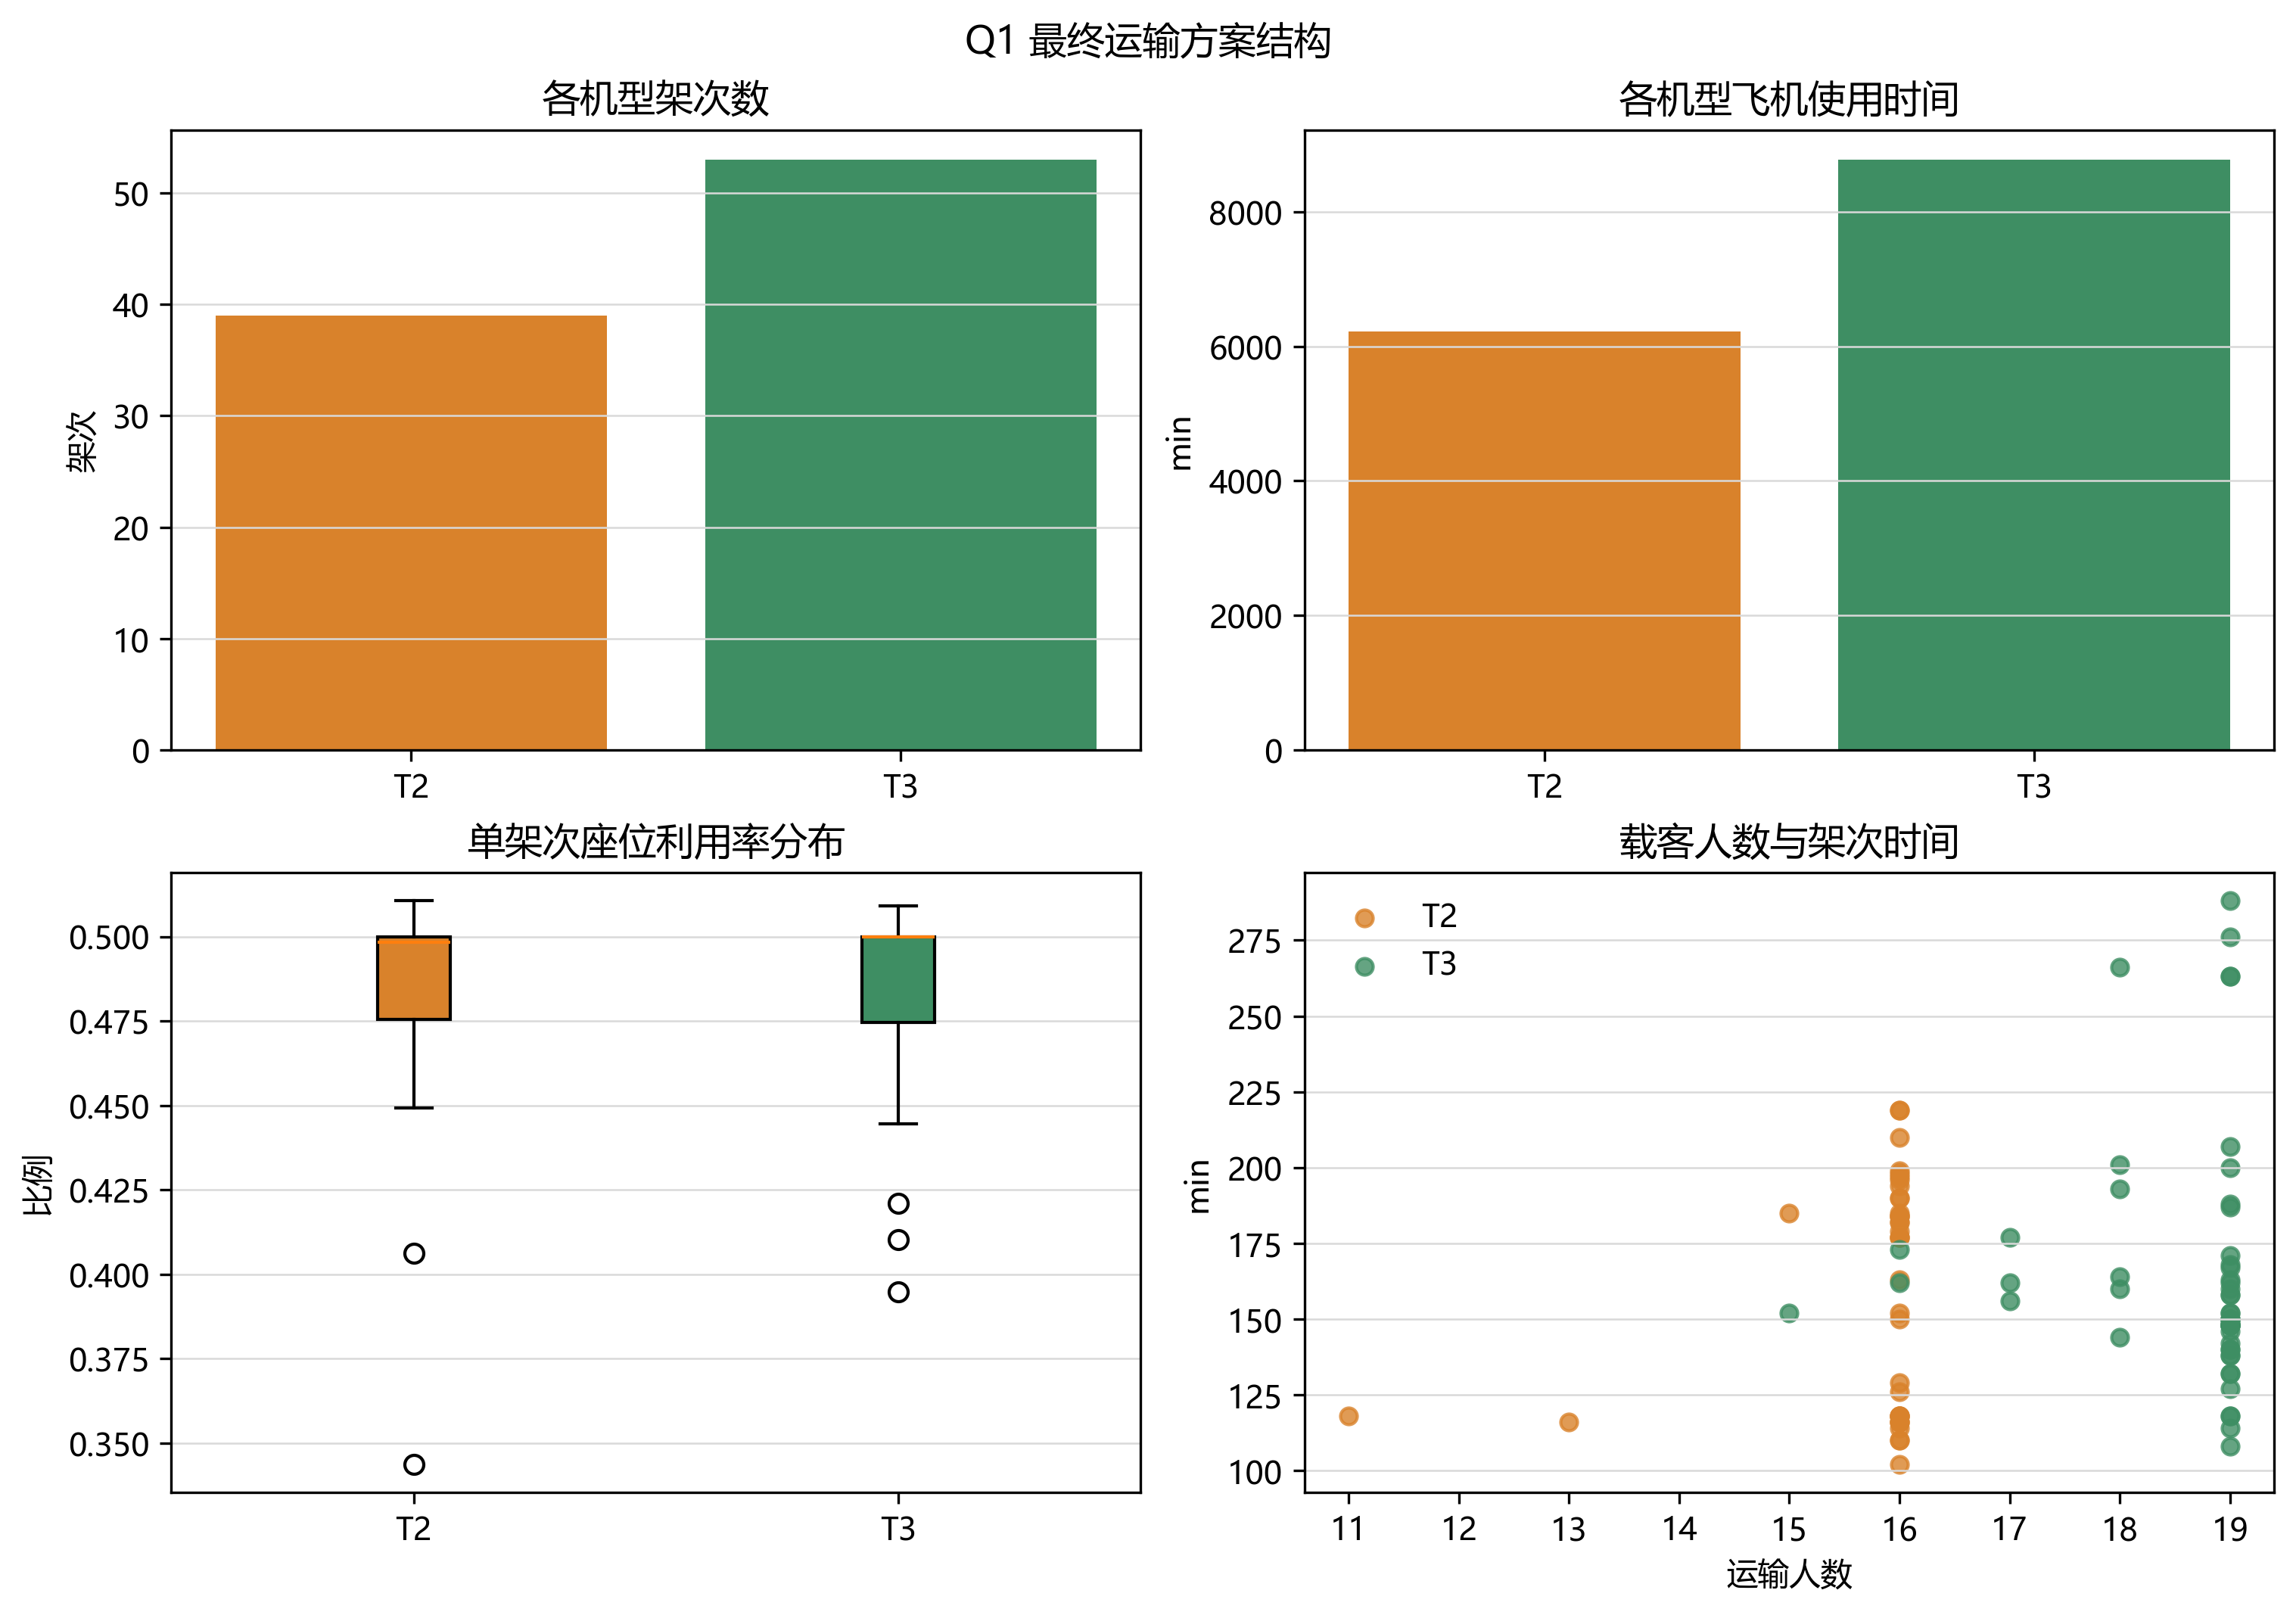
\includegraphics[width=0.8\linewidth]{outputs/figures/q1-route-profile.png}
    \caption{问题一的方案结构}
    \label{fig:placeholder}
\end{figure}

搜索过程指标演化如下所示
\begin{figure}[H]
    \centering
    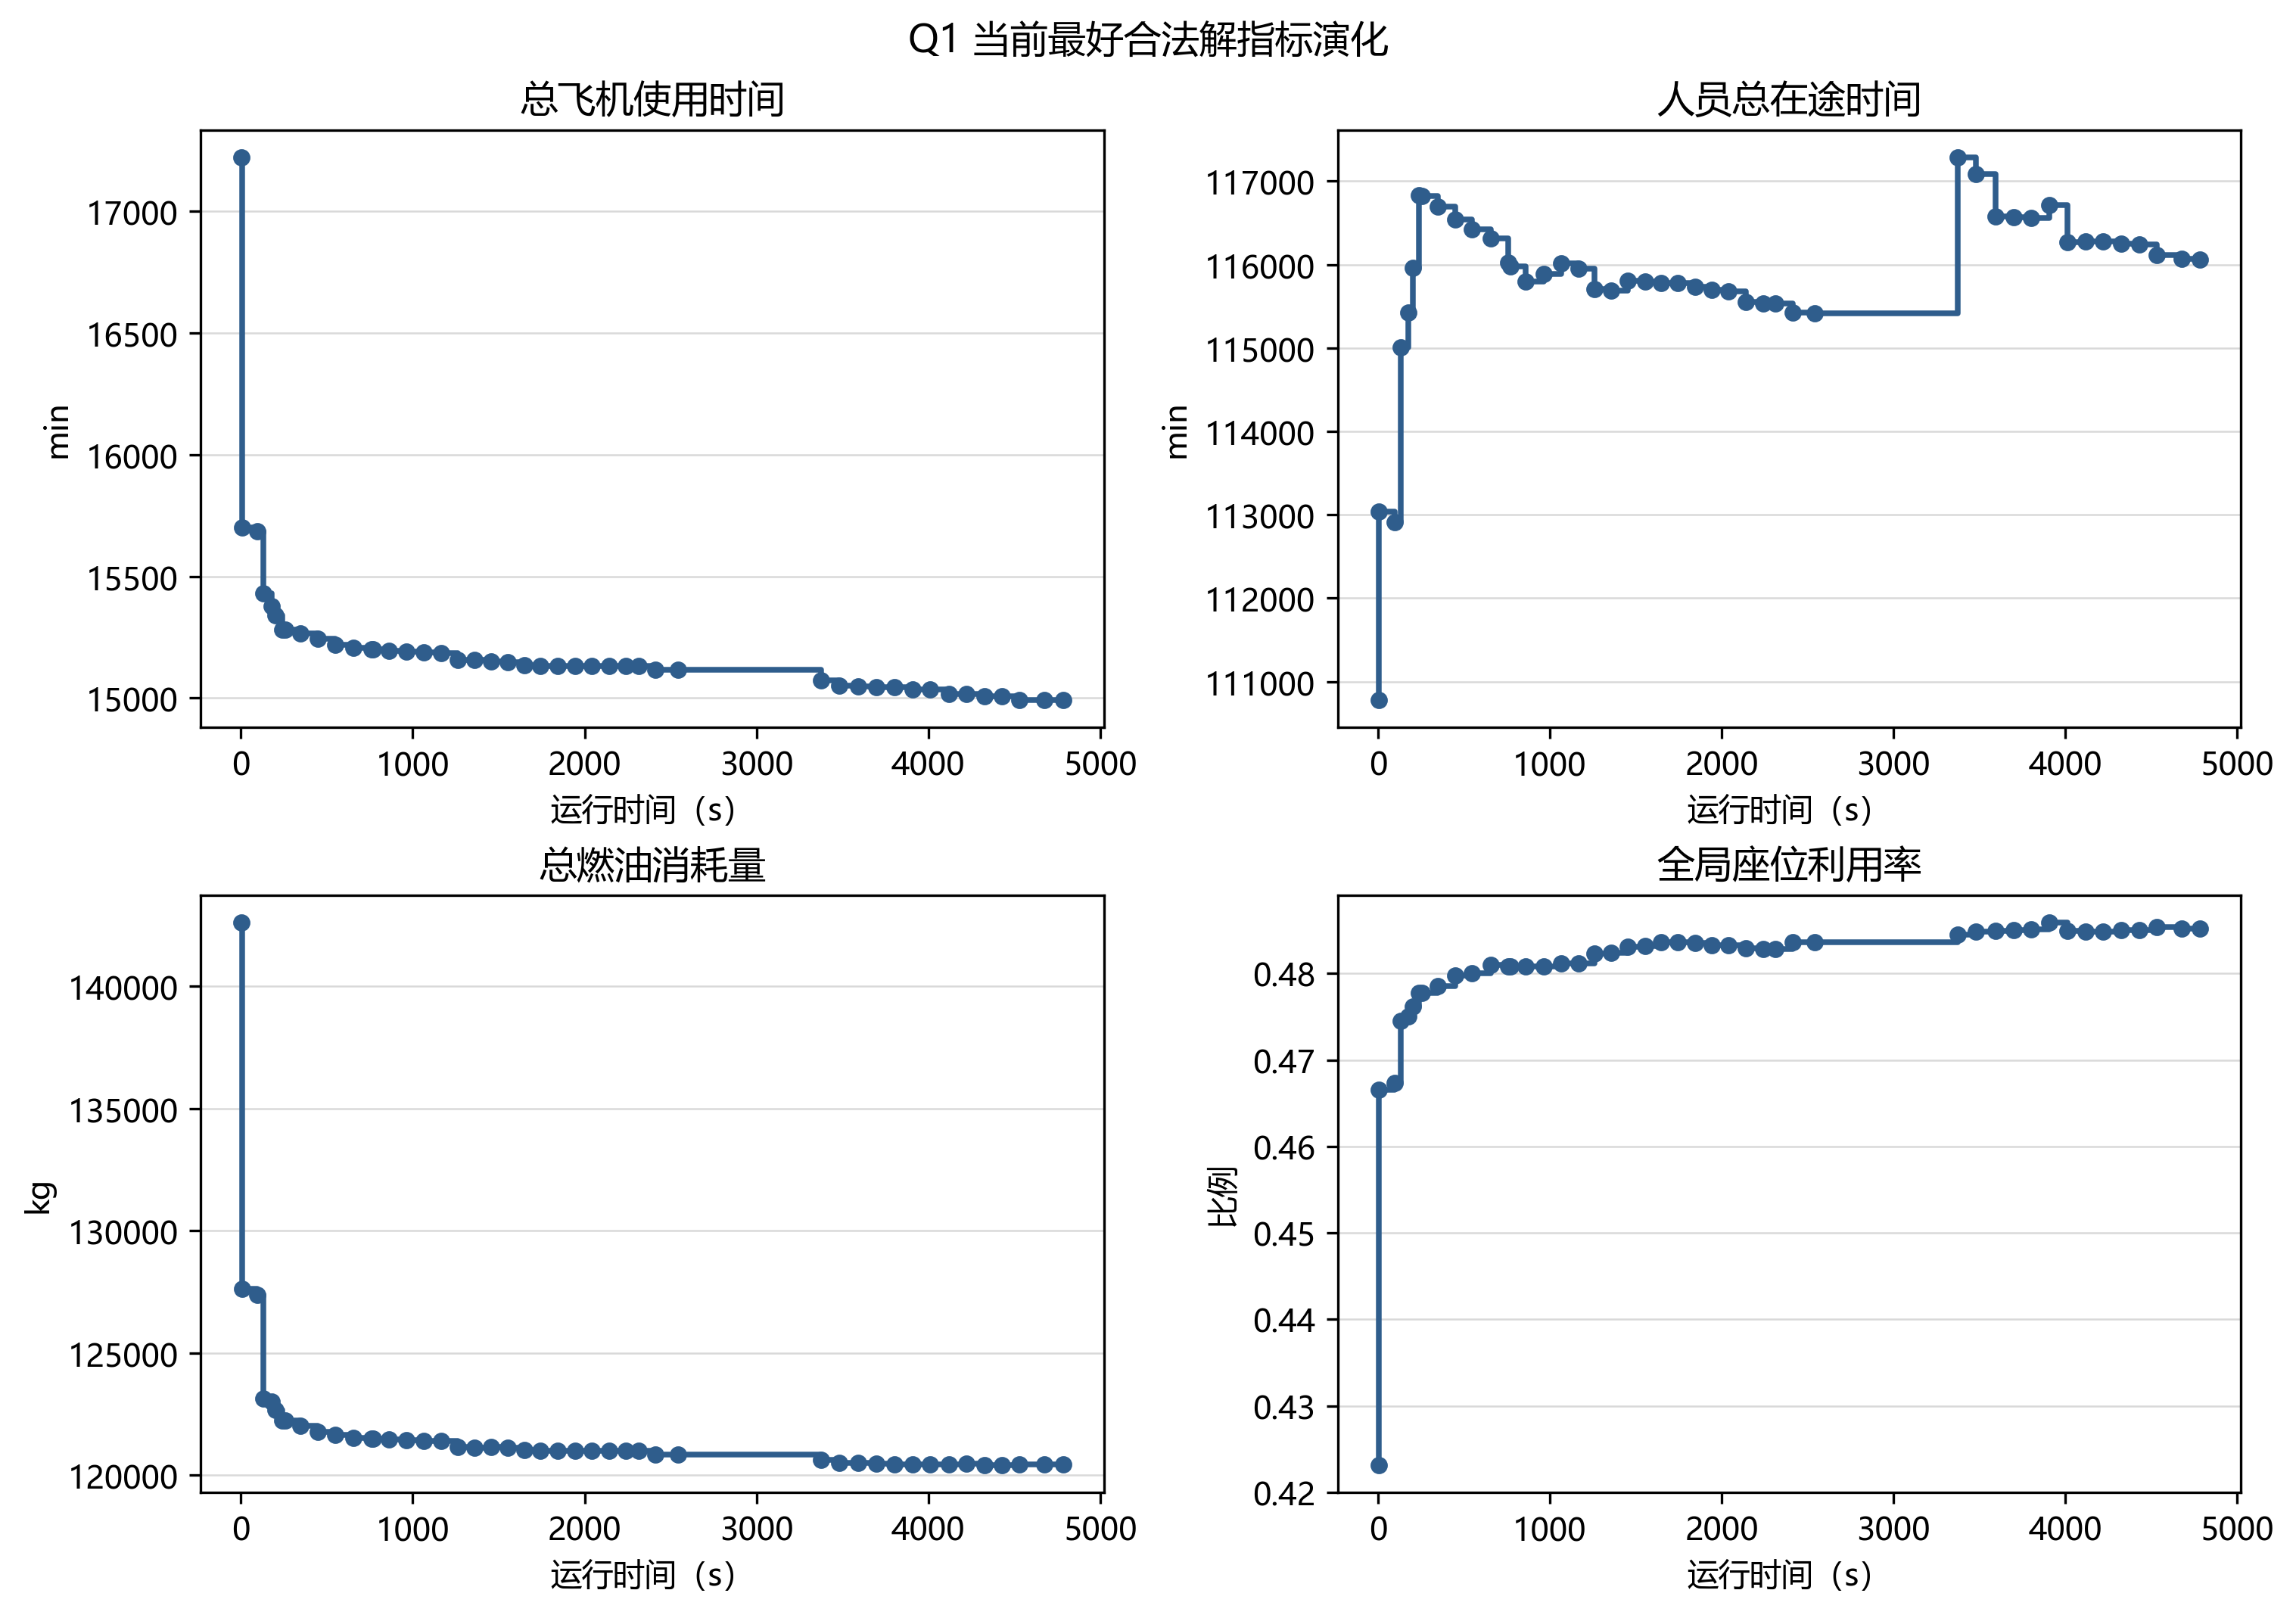
\includegraphics[width=0.8\linewidth]{outputs/figures/q1-convergence.png}
    \caption{各指标演化过程示意图}
    \label{fig:placeholder}
\end{figure}

\subsection{问题二的模型建立与求解}
\subsubsection{需求聚合与架次表示}

按人员的有向起终点将4000条需求划分为集合 $G$，其中出海1600人、海返1600人、设施间穿梭800人，共形成264个 OD 类。记第 $g$ 类人数为 $n_g$。聚合只用于路线搜索；最终仍将每一名人员映射回具体架次和上下机序号。

一条候选架次模板记为
\begin{equation}
 r=\left(a_r,k_r,v_{r0},v_{r1},\ldots,v_{r,m_r},v_{r,m_r+1}\right),
\end{equation}
其中 $a_r$ 为起降机场，$k_r\in\{T1,T2,T3\}$ 为机型，且
\begin{equation}
 v_{r0}=v_{r,m_r+1}=a_r,\qquad m_r\leq 5.
\end{equation}
中间节点 $v_{r1},\ldots,v_{r,m_r}$ 为实际停靠的海上设施，允许同一设施重复出现，每次出现均计为一次着陆。若需求明确指定机场，则 $a_r$ 必须与该机场一致；LAND 则绑定为模板所选机场。

设 $p_{rg}$、$d_{rg}$ 分别为 OD 类 $g$ 在模板 $r$ 中的上机与下机序号，则
\begin{equation}
 0\leq p_{rg}<d_{rg}\leq m_r+1.
\end{equation}
对于海上终点，下机序号取上机后第一次到达该终点的位置。这一约束既符合结果文件要求，也排除了人员到达目的地后继续随飞机绕行的无效安排。

\subsubsection{单架次时间、容量与燃油约束}

设地点 $u$ 到 $v$ 的距离为 $D_{uv}$。按照题意向上取整，机型 $k$ 在该航段的飞行时间为
\begin{equation}
 \tau_{uv}^{k}=\left\lceil\frac{60D_{uv}}{v_k}\right\rceil .
\end{equation}
令 $z_{rj}\in\{0,1\}$ 表示模板 $r$ 在第 $j$ 个海上停靠点是否加油，则该点停靠时间为
\begin{equation}
 s_{rj}=10+10z_{rj}.
\end{equation}
只有8座指定加油设施允许 $z_{rj}=1$。由此，模板的飞机使用时间为
\begin{equation}
 T_r=\sum_{j=0}^{m_r}\tau_{v_{rj},v_{r,j+1}}^{k_r}
     +\sum_{j=1}^{m_r}s_{rj}.
\end{equation}

记模板 $r$ 在第 $\ell$ 个航段的载客量为
\begin{equation}
 L_{r\ell}=\sum_{g\in G}q_{rg}
 \mathbf 1\!\left(p_{rg}\leq \ell<d_{rg}\right),
 \qquad \ell=0,1,\ldots,m_r,
\end{equation}
其中 $q_{rg}$ 表示模板 $r$ 运送第 $g$ 类人员的数量。同一停靠点先下后上，因此容量只需按离开该点后的航段检查：
\begin{equation}
 0\leq L_{r\ell}\leq Q_{k_r}.
\end{equation}

设 $F_{r\ell}^{-}$、$F_{r\ell}^{+}$ 分别表示到达节点 $v_{r\ell}$ 后、完成可能的加油后的剩余燃油。架次从机场满油起飞，即 $F_{r0}^{+}=C_{k_r}$。逐航段递推为
\begin{align}
 F_{r,ell+1}^{-}
 &=F_{r\ell}^{+}-b_{k_r}D_{v_{r\ell},v_{r,ell+1}},\\
 F_{r,ell+1}^{-}&\geq R_{k_r},\\
 F_{rell}^{+}
 &=z_{r\ell}C_{k_r}+(1-z_{r\ell})F_{r\ell}^{-},
 \qquad \ell=1,\ldots,m_r.
\end{align}
最终返回机场时同样满足最低安全余油约束。模板燃油消耗量为
\begin{equation}
 B_r=b_{k_r}\sum_{\ell=0}^{m_r}D_{v_{r\ell},v_{r,ell+1}}.
\end{equation}

记 $A_{rj}$、$E_{rj}$ 为模板到达和离开第 $j$ 个停靠位置的相对时刻，则模板内人员总在途时间、客座公里和可用座公里分别为
\begin{align}
 H_r&=\sum_{g\in G}q_{rg}\left(A_{r,d_{rg}}-E_{r,p_{rg}}\right),\\
 P_r&=\sum_{\ell=0}^{m_r}L_{r\ell}D_{v_{r\ell},v_{r,ell+1}},\\
 A_r&=Q_{k_r}\sum_{\ell=0}^{m_r}D_{v_{r\ell},v_{r,ell+1}}.
\end{align}

\subsubsection{路线池集合划分模型}

对每一种人员组合，路线生成器依次枚举满足穿梭取送先后关系的停靠序列、可选机场、三种机型及加油方案，并利用上述逐航段约束筛除不可行模板。服务设施不重复时完整枚举其顺序；仅当所有简单序列均不可行时，才在5次海上着陆范围内受控枚举设施重复序列，以处理相反方向穿梭或容量冲突。

设 $\mathcal R$ 为已生成的可行模板集合，$x_r\in\mathbb Z_{+}$ 表示模板 $r$ 被采用的次数。所有人员必须且只能运输一次，因此主问题的覆盖约束为
\begin{equation}
 \sum_{r\in\mathcal R}q_{rg}x_r=n_g,
 \qquad \forall g\in G.
\end{equation}

为保证总飞机使用时间具有绝对优先级，本文不将多个指标加权求和，而采用严格字典序求解：
\begin{equation}
 \operatorname{lexmin}
 \left(
 \sum_{r\in\mathcal R}T_rx_r,
 \sum_{r\in\mathcal R}H_rx_r,
 \sum_{r\in\mathcal R}B_rx_r,
 -\eta
 \right),
\end{equation}
其中
\begin{equation}
 \eta=
 \frac{\sum_{r\in\mathcal R}P_rx_r}
 {\sum_{r\in\mathcal R}A_rx_r}.
\end{equation}
求解时先得到最小飞机使用时间 $T^{*}$，再加入等式
$\sum_rT_rx_r=T^{*}$；随后依次固定人员总在途时间和燃油消耗量的最优值。最后采用分式规划迭代，将座位利用率目标转化为
\begin{equation}
 \max_{x}\left\{
 \sum_{r\in\mathcal R}P_rx_r-lambda
 \sum_{r\in\mathcal R}A_rx_r
 \right\},
\end{equation}
并更新 $\lambda$，直至分式目标不再改善。该过程保证低层目标不会以牺牲高层目标为代价。

\subsubsection{自适应大邻域候选生成与全局重组}

算法首先对每个 OD 类分别求解整数打包问题，得到保证可行的直接运输初解；再按路线间距离、共有设施和合并后的时间节约选择邻近路线，实施节约合并。该方案用于初始化路线池和整数主问题。

为了跳出局部合并结构，在当前主问题解上循环使用以下五类候选生成算子：
\begin{enumerate}
    \item \textbf{合并：}将两条路线的需求合并为一条路线；
    \item \textbf{转移：}从一条路线向另一条路线转移1至3名同类人员；
    \item \textbf{交换：}在两条路线间交换不同 OD 类的少量人员；
    \item \textbf{二路线重分配：}打散两条路线的需求并重新分为两组；
    \item \textbf{三路线压缩：}将三条路线的需求重新组织为两条可行路线。
\end{enumerate}
新生成的路线经单架次路线生成器验证后加入路线池，每轮再求解一次集合划分主问题，由主问题从全部历史候选中重新组合，而不是只接受局部替换。算子权重按照
\begin{equation}
 w_o\leftarrow0.85w_o+0.15R_o
\end{equation}
自适应更新，其中 $R_o$ 根据算子产生的新路线数、新路线是否进入主问题解以及本轮是否改进当前最好解确定。这样既保留有效算子，又避免搜索长期集中于单一邻域。

\subsubsection{模型求解结果}

程序在 Python 3.11 环境下实现，单架次路线由枚举与深度优先搜索生成，集合划分主问题由 OR-Tools CP-SAT 求解。4000名人员被聚合为264个 OD 类，最终路线池包含8478条候选模板。所得方案的主要指标见表~\ref{tab:q2-result}。

\begin{table}[htbp]
\centering
\caption{问题二运载方案主要指标}
\label{tab:q2-result}
\begin{tabular}{lc}
\toprule
指标 & 结果 \\
\midrule
总飞机使用时间 & 20751 min（345.85 h） \\
人员总在途时间 & 248493 min（4141.55 h） \\
总架次数 & 118 \\
总燃油消耗量 & 161473.10 kg \\
座位利用率 & 76.8449\% \\
\bottomrule
\end{tabular}
\end{table}

不同机型的架次构成见表~\ref{tab:q2-type}。T2与T3承担了绝大多数任务，其中T3座位数较多，适合需求较密集的联合运输；T2的单位距离油耗较低，在中等载客量路线中具有优势。该解释仅用于说明最终方案构成，机型选择本身由四层目标和逐航段约束共同决定。

\begin{table}[htbp]
\centering
\caption{问题二各机型架次数}
\label{tab:q2-type}
\begin{tabular}{cccc}
\toprule
机型 & T1 & T2 & T3 \\
\midrule
架次数 & 4 & 52 & 62 \\
\bottomrule
\end{tabular}
\end{table}

为观察路线池扩充后的收敛情况，表~\ref{tab:q2-convergence}列出部分迭代结果。第8轮产生的新路线使总飞机使用时间由20778分钟降至20751分钟；此后路线池继续由6868条扩充至8478条，四项指标均未再变化。

\begin{table}[htbp]
\centering
\caption{问题二路线池重组的收敛过程}
\label{tab:q2-convergence}
\begin{tabular}{ccccc}
\toprule
迭代轮次 & 路线池规模 & 飞机时间/min & 人员在途时间/min & 燃油/kg \\
\midrule
0  & 5834 & 20778 & 248626 & 161899.50 \\
8  & 6868 & 20751 & 248493 & 161473.10 \\
20 & 8478 & 20751 & 248493 & 161473.10 \\
\bottomrule
\end{tabular}
\end{table}

最终对输出结果进行独立回放校验：4000名人员均恰好出现一次；每名人员的上机位置早于下机位置，并在上机后第一次到达终点时下机；每个航段载客量不超过机型容量；每个架次海上着陆不超过5次；加油只发生在指定设施，且飞机到达每个节点及最终返场时均满足最低安全余油要求。上述检查全部通过。

每轮集合划分的四个目标阶段均返回 OPTIMAL，因此最终方案在已生成的8478条路线池内达到严格字典序最优。由于算法未枚举原问题的全部可行人员组合与路线，本文不据此声称获得原始完整路线空间上的全局最优解；后20轮中目标值保持不变，可作为当前候选生成范围内解已趋于稳定的数值证据。


\subsection{问题三的模型建立与求解}
\subsubsection{时空需求与架次表示}

问题三在问题二取送联合运输模型的基础上增加人员时间窗、业务类型和具体飞机资源。将规划期起点2026年8月3日00:00记为时刻0，全部时间统一换算为整数分钟。设全部人员集合为$I$，其中应急取送、生产倒班和常规倒班人员构成必需人员集合$I^{M}$，临时人员构成集合$I^{T}$，满足

\begin{equation}
I=I^{M}\cup I^{T},
\qquad
I^{M}\cap I^{T}=\varnothing.
\end{equation}

对人员$i\in I$，记起点、终点、最早可离开时刻和最晚到达时刻分别为$o_i$、$d_i$、$E_i$和$L_i$。与问题二不同，即使多名人员具有相同OD，其时间窗也可能不同，因此候选路线必须保存具体的人员编号，而不能只保存OD聚合人数。

因此我们将一条问题三候选架次表示为

\begin{equation}
r=
\left(
I_r,\,
a_r,\,
k_r,\,
v_{r0},v_{r1},\ldots,v_{r,m_r},v_{r,m_r+1},\,
\boldsymbol{\rho}_r,\,
\mathcal{I}_r
\right),
\end{equation}

其中，$I_r$为架次运输的具体人员集合，$a_r$为起降机场，$k_r$为机型，$v_{rj}$为第$j$个停靠位置，$\rho_{rj}\in\{0,1\}$表示是否在第$j$个海上设施加油，$\mathcal{I}_r$为该架次的可行起飞时刻集合。架次必须从同一机场起飞并返场，且海上着陆不超过5次，即

\begin{equation}
v_{r0}=v_{r,m_r+1}=a_r,
\qquad
a_r\in\{\mathrm{A01},\mathrm{A02},\mathrm{A03}\},
\qquad
m_r\leq 5.
\end{equation}

若人员的起点或终点明确指定为某一机场，则$a_r$必须与该机场一致；若相应地点为LAND，则由架次实际选择的机场$a_r$确定。

设$p_{ir}$和$d_{ir}$分别为人员$i$在架次$r$中的上机和下机序号，则有

\begin{equation}
0\leq p_{ir}<d_{ir}\leq m_r+1.
\end{equation}

对于终点为海上设施的人员，必须在上机后第一次到达该设施时下机，即

\begin{equation}
d_{ir}
=
\min
\left\{
j\mid j>p_{ir},\ v_{rj}=d_i
\right\}.
\end{equation}

通过这些约束可以保证取送先后关系、人员不换乘以及到达目的地后立即下机的要求。

\subsubsection{单架次时间、容量与燃油约束}

设地点$u$到$v$的距离为$D_{uv}$，机型$k$的速度、座位数、单位距离油耗、油箱容量和最低安全余油分别为$v_k$、$Q_k$、$b_k$、$C_k$和$R_k$。则对应航段的飞行时间向上取整为

\begin{equation}
\tau_{uv}^{k}
=
\left\lceil
\frac{60D_{uv}}{v_k}
\right\rceil.
\end{equation}

普通停靠时间为10分钟，加油停靠时间为20分钟，因此架次$r$在第$j$个海上设施的停靠时间为

\begin{equation}
g_{rj}=10+10\rho_{rj}.
\end{equation}

若记$\alpha_{rj}$和$\beta_{rj}$分别为相对于起飞时刻的到达和离开时刻。则各节点时刻按照

\begin{equation}
\begin{aligned}
&\alpha_{r0}=\beta_{r0}=0,\\
&\alpha_{r,j+1}
=
\beta_{rj}
+
\tau_{v_{rj},v_{r,j+1}}^{k_r},
\qquad j=0,1,\ldots,m_r,\\
&\beta_{rj}
=
\alpha_{rj}+g_{rj},
\qquad j=1,2,\ldots,m_r
\end{aligned}
\end{equation}

逐段递推计算。可以得到架次$r$的飞机使用时间为

\begin{equation}
T_r=\alpha_{r,m_r+1}.
\end{equation}

由于到达每个设施后先下客、后上客。因此第$\ell$个航段的载客人数为

\begin{equation}
L_{r\ell}
=
\sum_{i\in I_r}
\mathbf{1}
\left(
p_{ir}\leq \ell<d_{ir}
\right),
\qquad
\ell=0,1,\ldots,m_r,
\end{equation}

并满足逐航段容量约束

\begin{equation}
0\leq L_{r\ell}\leq Q_{k_r},
\qquad
\ell=0,1,\ldots,m_r.
\end{equation}

设$F_{rj}^{+}$和$F_{r,j+1}^{-}$分别为离开位置$j$及到达下一位置时的剩余燃油。飞机从机场满油起飞，则燃油量可以按照下式递推：

\begin{equation}
\begin{aligned}
&F_{r0}^{+}=C_{k_r},\\
&F_{r,j+1}^{-}
=
F_{rj}^{+}
-
b_{k_r}D_{v_{rj},v_{r,j+1}},\\
&F_{r,j+1}^{-}\geq R_{k_r},\\
&F_{rj}^{+}
=
\rho_{rj}C_{k_r}
+
(1-\rho_{rj})F_{rj}^{-}.
\end{aligned}
\end{equation}
其中，仅当$v_{rj}$为指定加油设施时才允许$\rho_{rj}=1$。所以架次$r$的燃油消耗量为

\begin{equation}
B_r
=
b_{k_r}
\sum_{j=0}^{m_r}
D_{v_{rj},v_{r,j+1}}.
\end{equation}

设架次$r$的实际起飞时刻为$s_r$。人员$i$的实际离开起点时刻和到达终点时刻分别为$s_r+\beta_{r,p_{ir}}$和$s_r+\alpha_{r,d_{ir}}$，故时间窗约束为

\begin{equation}
s_r+\beta_{r,p_{ir}}\geq E_i,
\qquad
s_r+\alpha_{r,d_{ir}}\leq L_i.
\end{equation}
由此推出该架次起飞时刻的共同上下界为

\begin{equation}
\underline{s}_r
=
\max_{i\in I_r}
\left\{
E_i-\beta_{r,p_{ir}}
\right\},
\qquad
\overline{s}_r
=
\min_{i\in I_r}
\left\{
L_i-\alpha_{r,d_{ir}}
\right\}.
\end{equation}

设第$q$天从时刻$1440q$开始。结合06:00至18:00起飞及20:00前返场的要求，架次$r$在第$q$天的可行起飞区间为
\begin{equation}
\mathcal{I}_{rq}
=
\left[
\max
\left\{
\underline{s}_r,\,
1440q+360
\right\},
\,
\min
\left\{
\overline{s}_r,\,
1440q+1080,\,
1440q+1200-T_r
\right\}
\right].
\end{equation}
删除空区间，整个规划期内的可行起飞时刻集合为

\begin{equation}
\mathcal{I}_r
=
\bigcup_{q=0}^{6}
\mathcal{I}_{rq}.
\end{equation}

只有当$\mathcal{I}_r\neq\varnothing$时，该架次才加入时空路线池。这样就将人员时间窗、机场运行时间和当天返场要求统一压缩为候选架次的可行起飞区间。

最后再表示出架次$r$的人员总在途时间、客座公里和可用座公里

\begin{equation}
\begin{aligned}
H_r
&=
\sum_{i\in I_r}
\left(
\alpha_{r,d_{ir}}
-
\beta_{r,p_{ir}}
\right),\\
P_r
&=
\sum_{\ell=0}^{m_r}
L_{r\ell}D_{v_{r\ell},v_{r,\ell+1}},\\
A_r
&=
Q_{k_r}
\sum_{\ell=0}^{m_r}
D_{v_{r\ell},v_{r,\ell+1}}.
\end{aligned}
\end{equation}

\subsubsection{具体飞机排班与两阶段优化模型}

设$\mathcal{R}$为已生成的时空候选架次集合，$\mathcal{H}_{ak}$为属于机场$a$且机型为$k$的具体飞机集合。定义$z_r\in\{0,1\}$表示是否执行架次$r$，$x_{rh}\in\{0,1\}$表示是否由具体飞机$h$执行架次$r$，则

\begin{equation}
\sum_{h\in\mathcal{H}_{a_rk_r}}
x_{rh}
=
z_r,
\qquad
r\in\mathcal{R}.
\end{equation}
保证每个被选架次恰好分配给一架机场和机型均相容的飞机。并且每名必需人员必须且只能运输一次。而对于临时人员$i\in I^{T}$，定义$y_i\in\{0,1\}$表示是否成功运输，则有

\begin{equation}
\sum_{r\in\mathcal{R}:i\in I_r}
z_r
=
y_i,
\qquad
i\in I^{T}.
\end{equation}

架次起飞时刻满足$s_r\in\mathcal{I}_r$。若架次$r$由飞机$h$执行，则该架次对飞机资源的占用区间为$[s_r,s_r+T_r+30)$。对每架具体飞机设置不重叠约束

\begin{equation}
\operatorname{NoOverlap}
\left(
\left\{
[s_r,s_r+T_r+30):
x_{rh}=1
\right\}
\right),
\qquad
h\in\mathcal{H}.
\end{equation}

由此同时保证同一飞机的架次不发生重叠，并满足返场后至少30分钟的周转要求。

因此全部被选架次的总飞机使用时间、人员总在途时间、总架次数、燃油消耗量和座位利用率分别记为

\begin{equation}
\begin{aligned}
T&=\sum_{r\in\mathcal{R}}T_rz_r,\\
H&=\sum_{r\in\mathcal{R}}H_rz_r,\\
N&=\sum_{r\in\mathcal{R}}z_r,\\
F&=\sum_{r\in\mathcal{R}}B_rz_r,\\
\eta
&=
\frac{\displaystyle\sum_{r\in\mathcal{R}}P_rz_r}
{\displaystyle\sum_{r\in\mathcal{R}}A_rz_r}.
\end{aligned}
\end{equation}

在第一阶段仅安排 $I^{M}$ 中的人员，优化过程采用严格字典序目标 $\operatorname{lexmin}(T,H,N,F,-\eta)$。然后记第一阶段得到的最小总飞机使用时间为$B$。第二阶段加入临时人员后，在保持全部必需人员的精确覆盖约束的前提下，增加$T\leq B$的约束，临时人员完成数量记为

\begin{equation}
Y=\sum_{i\in I^{T}}y_i.
\end{equation}
由于第二阶段首先最大化临时人员完成数量，再依次优化其余运输指标，因此其严格字典序目标为 $\operatorname{lexmin}(-Y,T,H,N,F,-\eta)$。

\subsubsection{时空路线池生成与大邻域搜索}

在确定了单架次时空和机队排班模型的基础上，我们的思路是生成所有可行的时空路线加入路线池以供选择，并在搜索过程中逐渐扩充，重组来搜索最优情况。由于问题三中同一 OD 人员的时间窗可能存在明显差异，因此每条候选路线均绑定具体人员编号，并记录可执行日期、起降机场、机型、设施停靠顺序、上下机位置、加油方式及可行起飞时间区间。

首先在第一阶段，先按照有向 OD 和时间兼容关系构造初始人员批次。同一 OD 内部依次按照任务优先级、最晚到达时间和最早离开时间排序，再逐人尝试加入当前批次。若加入新人员后无法由任一机场和机型形成合法架次，则结束当前批次并建立新批次。该过程保证每名非临时人员至少具有一条时间可行的基础路线。而对每种人员的组合，时空路线生成器依次枚举实际起降机场、机型、海上设施停靠顺序、取送位置等变量，并对每种枚举结果检查动态载客量、取送先后关系、人员时间窗等约束。最终形成简单的初始路线池。

与问题一、二思路相近，通过枚举确定问题的初始路线池后。检查路线池，对时间相容且空间位置接近的两个批次进行合并，并随机尝试少量三批次联合运输。随后以当前主问题选中的路线为中心构造大邻域，合并设施位置接近且存在共同可执行日期的路线并将两条路线中的人员打散，再按照时间先后、交替分配和 OD 排序等方式重新分配形成新的组合，若检验为合法路线，则加入路线池，再由CP-SAT主问题进行全局重组。搜索结束后，计算得到的最佳总飞机使用时间，记为 $B$。

第二阶段则保留全部非临时人员的恰好覆盖约束，同时生成临时人员单独路线、同 OD 时间兼容以及可以将临时人员插入的候选路线。临时人员按照其起终点与当前路线设施集合的空间距离排序，优先尝试插入距离最近的路线，若两个临时人员均能分别插入，再尝试成对插入。在此过程中始终检查新情况是否满足 $T\leq B$约束，同时依据严格字典序目标 $\operatorname{lexmin}(-Y,T,H,N,F,-\eta)$搜索结果。

\subsubsection{模型求解结果}

实验中涉及参数变量的设置，我们的设置为总搜索时间上限3600秒，其中55\%的时间资源用于第一阶段；每次CP-SAT主问题的求解时间上限为180秒。路线池上限为15000条，第一阶段和第二阶段初始化时分别开放70\%和90\%的路线池容量，为后续邻域搜索保留扩充空间。具体参数见表~\ref{tab:q3-parameters}。

% 参数说明后立即插入参数表

\begin{table}[H]

\centering
\caption{问题三最终实验参数}
\label{tab:q3-parameters}
\small

\begin{tabular}{lll}

\toprule
参数 & 含义 & 取值 \\
\midrule
\texttt{time-limit} & 总搜索时间上限/s & 3600 \\
\texttt{stage1-fraction} & 第一阶段时间比例 & 0.55 \\
\texttt{master-time} & 单次主问题时间/s & 180 \\
\texttt{epochs} & 第一阶段LNS轮数 & 6 \\
\texttt{temp-epochs} & 第二阶段LNS轮数 & 5 \\
\texttt{ops-per-epoch} & 每轮重分包次数 & 30 \\
\texttt{neighbors} & 路线邻居数量 & 2 \\
\texttt{bootstrap-neighbors} & 初始批次合并邻居数 & 5 \\
\texttt{bootstrap-triples} & 三批次合并尝试数 & 100 \\
\texttt{temp-candidates-per-route} & 每条路线临时人员候选数 & 2 \\
\texttt{route-variants} & 每个人员组合保留路线数 & 4 \\
\texttt{max-patterns} & 路线池硬上限 & 15000 \\
\texttt{stage1-pool-fraction} & 第一阶段路线池比例 & 0.70 \\
\texttt{stage2-bootstrap-pool-fraction} & 第二阶段初始路线池比例 & 0.90 \\
\texttt{max-route-people} & 单次生成器最大候选人数 & 38 \\
\texttt{assignment-limit} & 上下机方案枚举上限 & 300 \\
\texttt{workers} & 并行线程数 & 8 \\
\texttt{seed} & 随机种子 & 2026 \\
\bottomrule

\end{tabular}

\end{table}

该参数是目前在多次参数调整中得到的综合最优结果，在初步实验中我们仅设置了2轮第一阶段LNS，并取路线邻居数为3，路线池上限为12000，并行线程数为4。该参数能够完成全部160名临时人员，但得到的第一阶段总飞机使用时间较长。考虑到题目要求优先考虑第一阶段总飞机使用时间的最小化，我们才将第一阶段LNS轮数由2轮提高到6轮，并增强了其他第一阶段参数来加强反馈过程和增加候选路线总量，优化了总飞机使用时间。不过由于增强了第一阶段的搜索强度，导致第二阶段可用的搜索时间减少，因此现结果无法满足全部临时人员的运输要求。经过考虑，我们选择保留现在总飞行时间更优的实验结果。调整前后的结果见表~\ref{tab:q3-tuning}。

% 调参思路后立即插入参数效果对比表

\begin{table}[H]

\centering
\caption{问题三参数调整前后的结果比较}
\label{tab:q3-tuning}
\small

\begin{tabular}{lrr}

\toprule
指标 & 初步参数 & 最终参数 \\
\midrule
第一阶段基准/min & 36040 & 32887 \\
临时人员完成数 & 160 & 154 \\
人员总在途时间/min & 264617 & 269475 \\
总架次数 & 178 & 164 \\
总燃油消耗量/kg & 274578.90 & 247971.70 \\
座位利用率 & 49.7182\% & 54.6549\% \\
最终路线池规模 & 11245 & 10832 \\
\bottomrule

\end{tabular}

\end{table}

两阶段搜索的收敛过程如图~\ref{fig:q3-convergence}所示。第一阶段初始路线池包含5106条候选路线，初始排班总飞机使用时间为52314分钟。经过6轮邻域扩充和主问题重组，第一阶段结束时路线池规模为6821，$B=32887$ 分钟。

% 第一阶段和第二阶段收敛分析后立即插入收敛图

\begin{figure}[H]

\centering
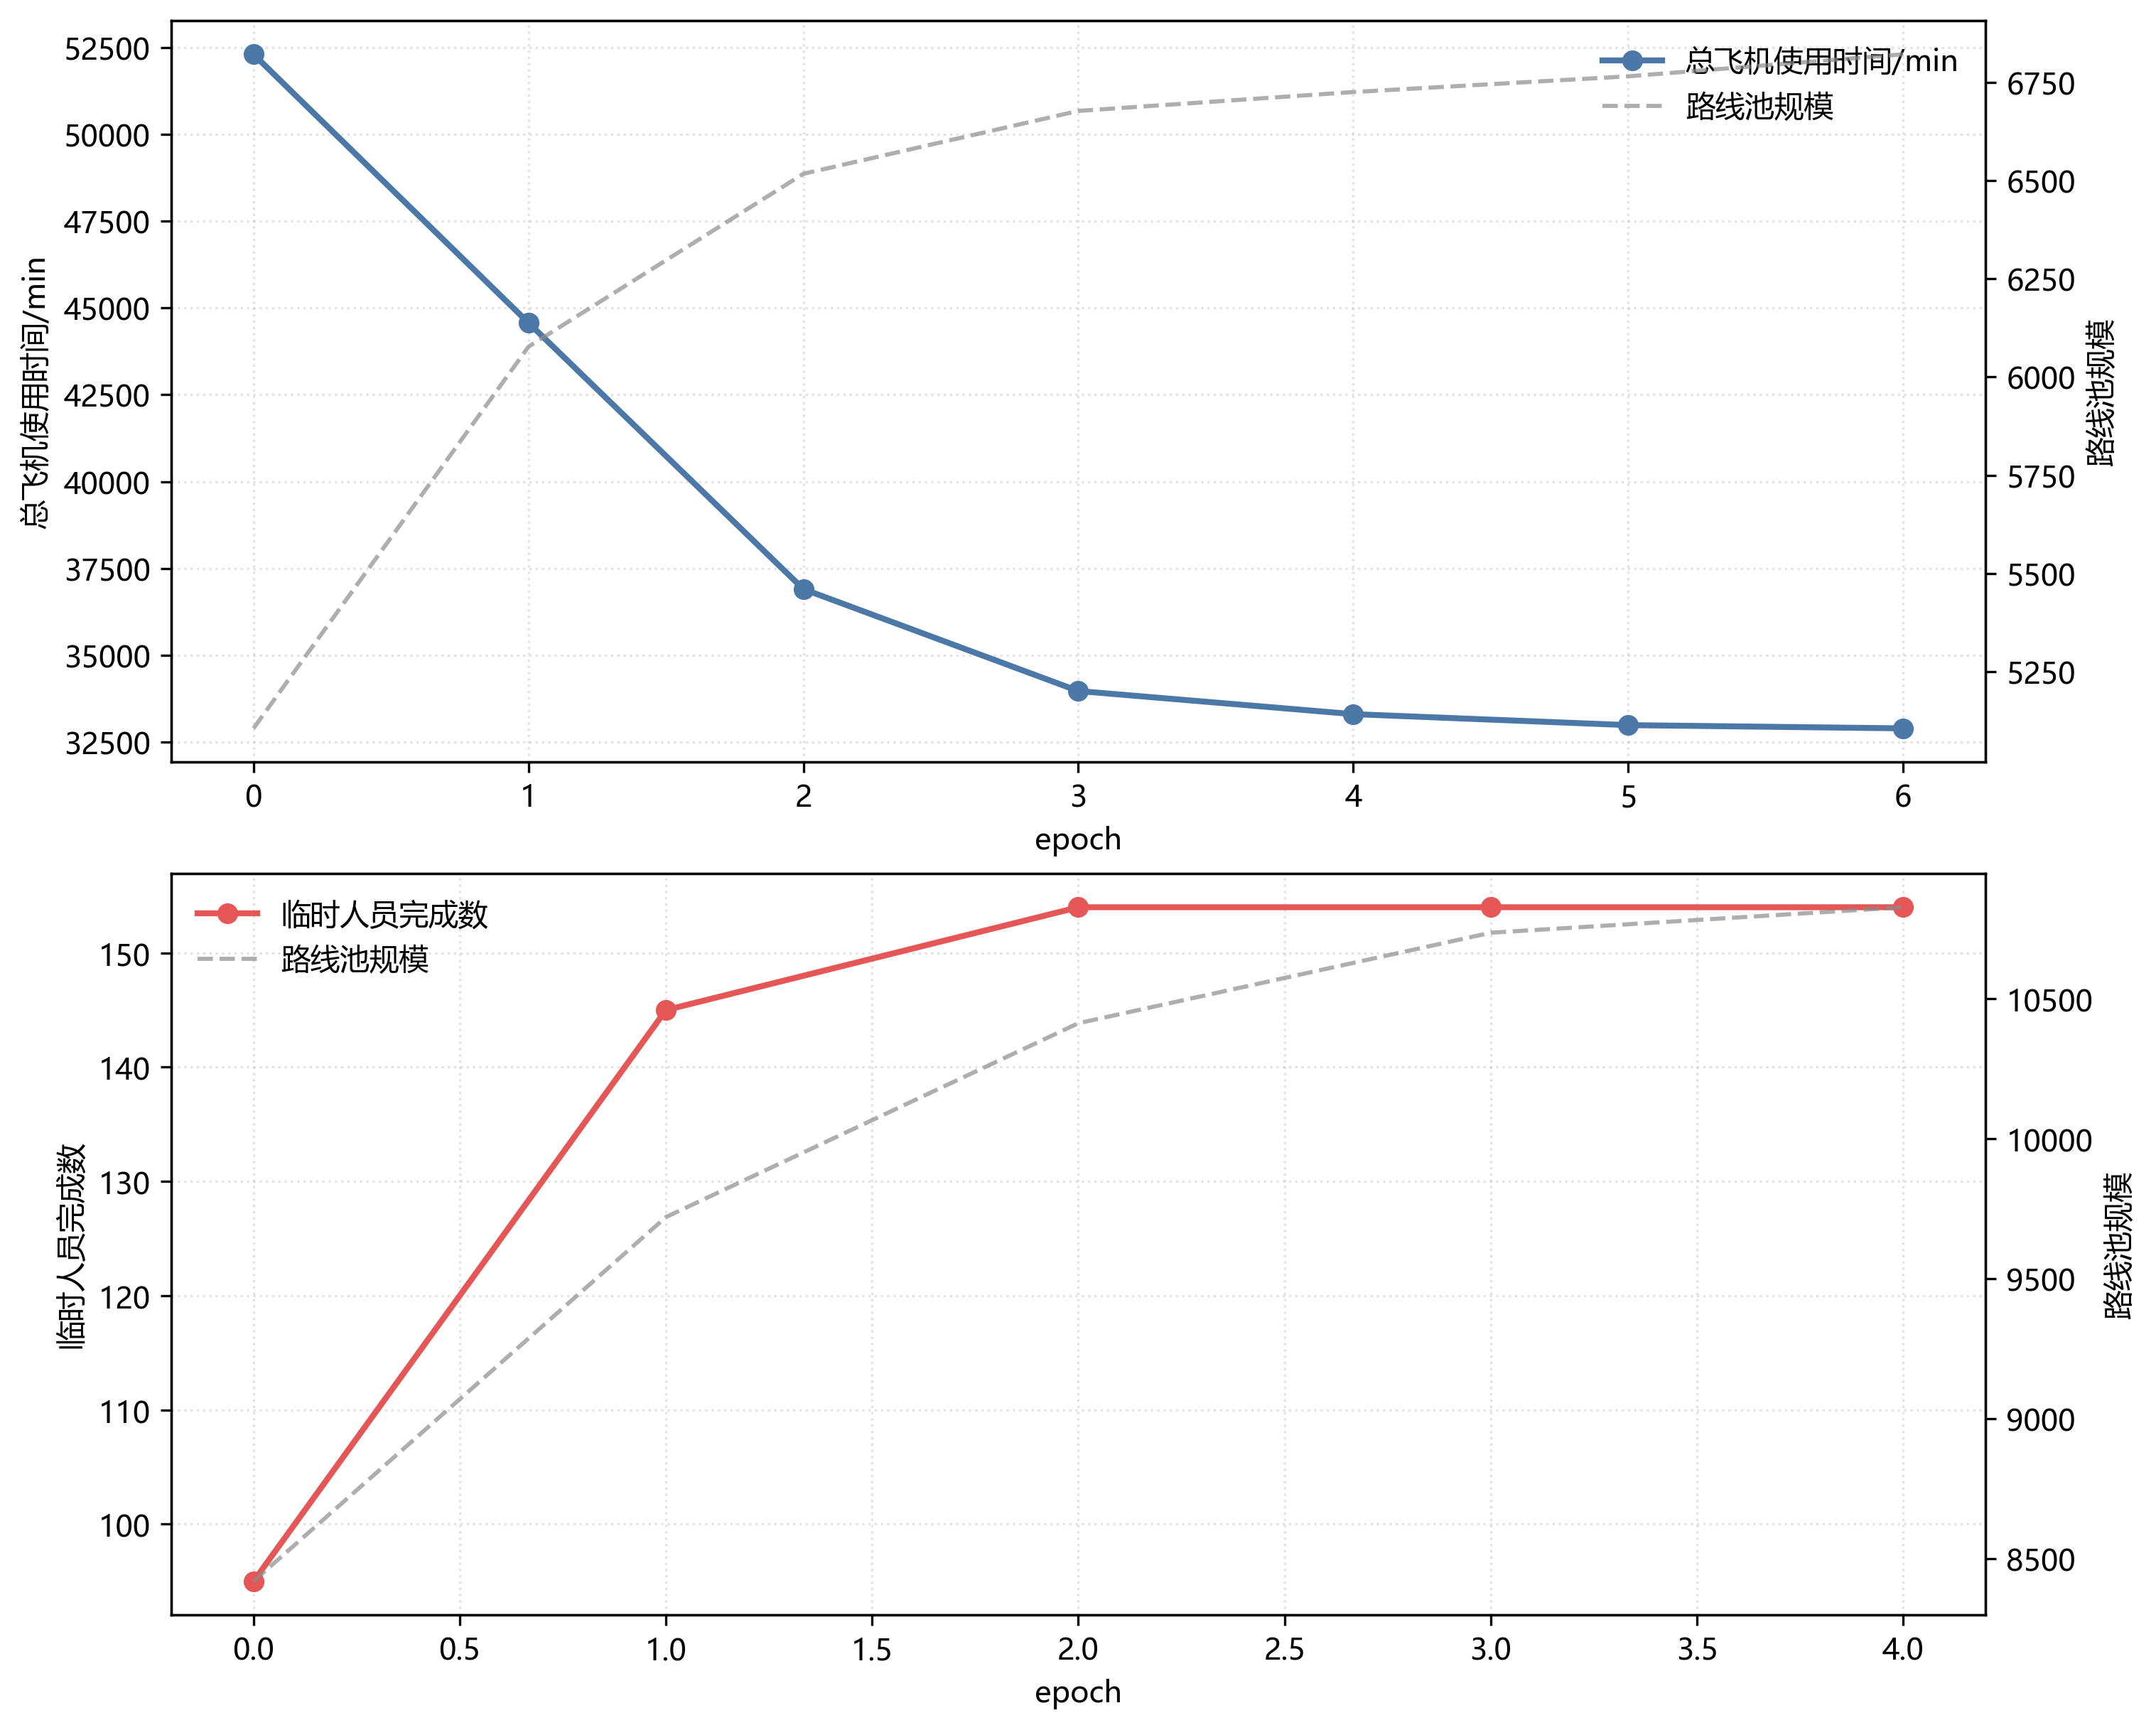
\includegraphics[width=0.78\textwidth]{outputs/figures/q3_two_stage_convergence.png}
\caption{问题三两阶段搜索收敛过程}
\label{fig:q3-convergence}

\end{figure}
因此最终方案能够完成全部40名应急处置人员、360名增储上产人员和3440名常规倒班人员，并\textbf{完成154名临时人员}，共运输3994人。第一阶段基准和第二阶段最终\textbf{总飞机使用时间均为32887分钟，即548.12小时，人员总在途时间269475分钟，总架次数164，总燃油消耗量267971.70kg，座位利用率54.6549\%}。说明几乎所有临时人员都能通过利用已有架次的空余座位和重组联合运输路线加入，无法加入的6位临时人员的临时任务只能为了减少运输开销而取消。最终方案主要指标见表~\ref{tab:q3-results}。

% 总体结果说明后立即插入结果表

\begin{table}[H]

\centering
\caption{问题三最终运输方案主要指标}
\label{tab:q3-results}

\begin{tabular}{lr}

\toprule
指标 & 结果 \\
\midrule
非临时人员完成数 & 3840/3840 \\
临时人员完成数 & 154/160 \\
临时任务满足率 & 96.25\% \\
第一阶段基准总飞机使用时间 & 32887 min（548.12 h） \\
最终总飞机使用时间 & 32887 min（548.12 h） \\
人员总在途时间 & 269475 min（4491.25 h） \\
总架次数 & 164 \\
总燃油消耗量 & 247971.70 kg \\
座位利用率 & 54.6549\% \\
路线池规模 & 10832 \\
\bottomrule

\end{tabular}

\end{table}

最终完成154名临时人员，另有6名临时人员未被安排。如图~\ref{fig:q3-temporary}所示，未完成的6名临时人员均为设施间穿梭人员，其时间窗宽度介于1930分钟至6565分钟，并未集中在时间窗最窄的区域。因此，这些人员未被安排的主要原因并不是单人时间窗过紧，而是在 $T\leq32887$ 的严格限制下，其起终点难以与当前非临时架次形成不增加飞机使用时间的联合运输结构。若为其增加独立架次或明显绕行，则会突破第一阶段时间基准。

% 临时人员满足情况解释后立即插入分析图

\begin{figure}[H]

\centering
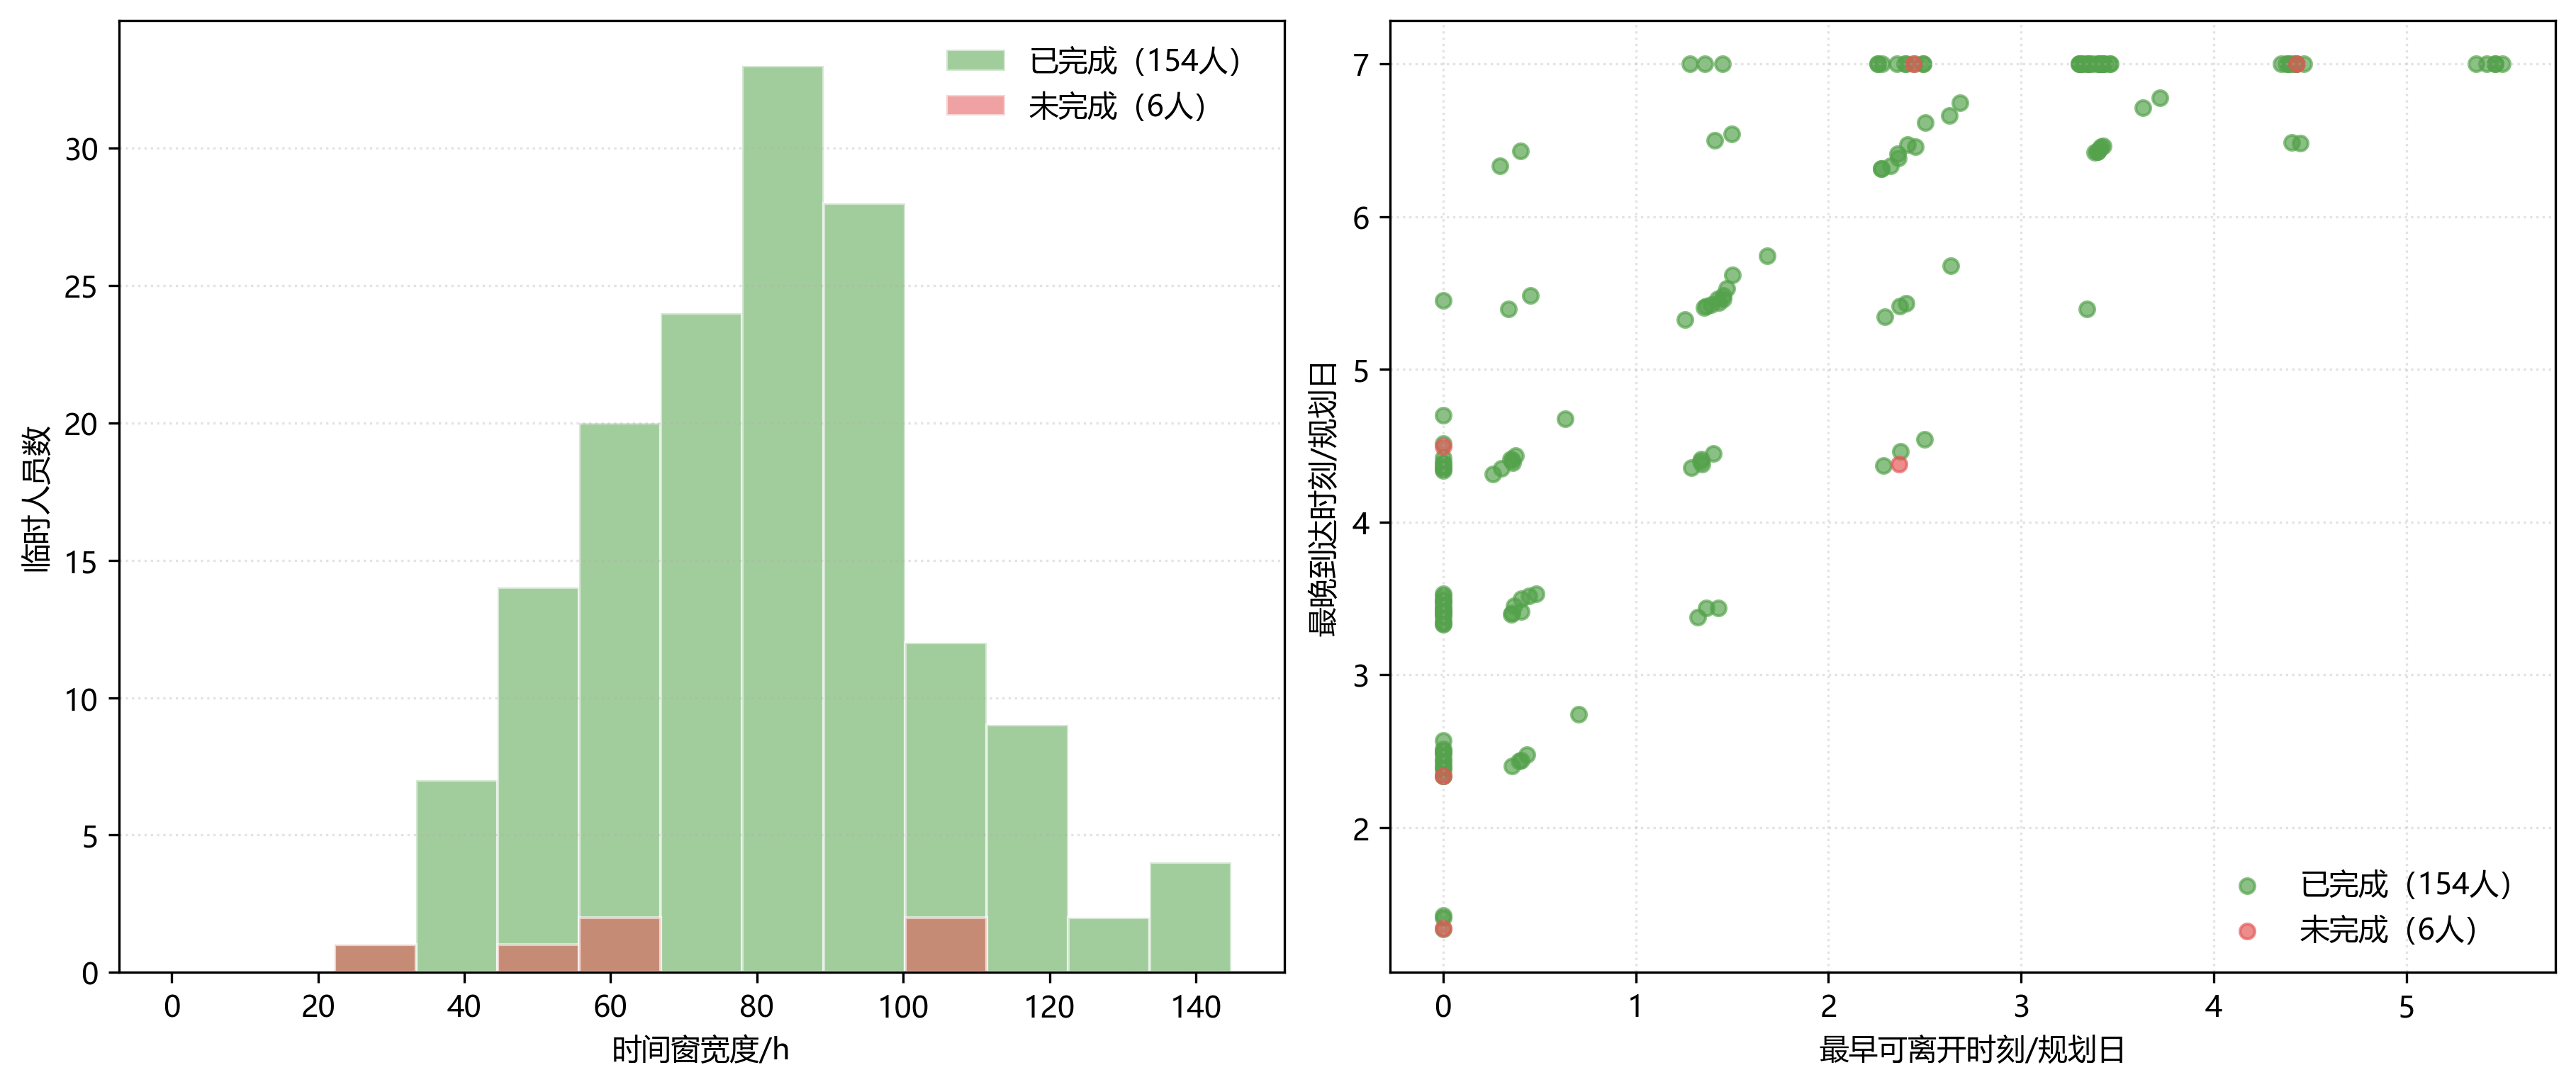
\includegraphics[width=0.92\textwidth]{outputs/figures/q3_temporary_service_analysis.png}
\caption{临时人员完成情况及其时间特征}
\label{fig:q3-temporary}

\end{figure}

分析最终结果的架次安排情况可以发现，在164个架次中，T1、T2和T3分别承担12、90和62个架次，对应飞机使用时间分别为1914、17356和13617分钟。T2承担的架次数最多，也说明其16座容量、较低单位距离油耗以及较大的配备数量，使其在有限机队排班中具有较好的综合适应性。规划期内共有21架具体飞机被实际使用。

48个存在实际任务的“日期—机场—机型”组合中，有36个组合的最大同时占用飞机数达到该组机队数量上限，表明T2和T3等局部机队资源在高负荷日期形成了实际约束。各日期、机场和机型的工作负荷见图~\ref{fig:q3-workload}。

% 每日机场工作负荷分析后立即插入柱状图

\begin{figure}[H]

\centering
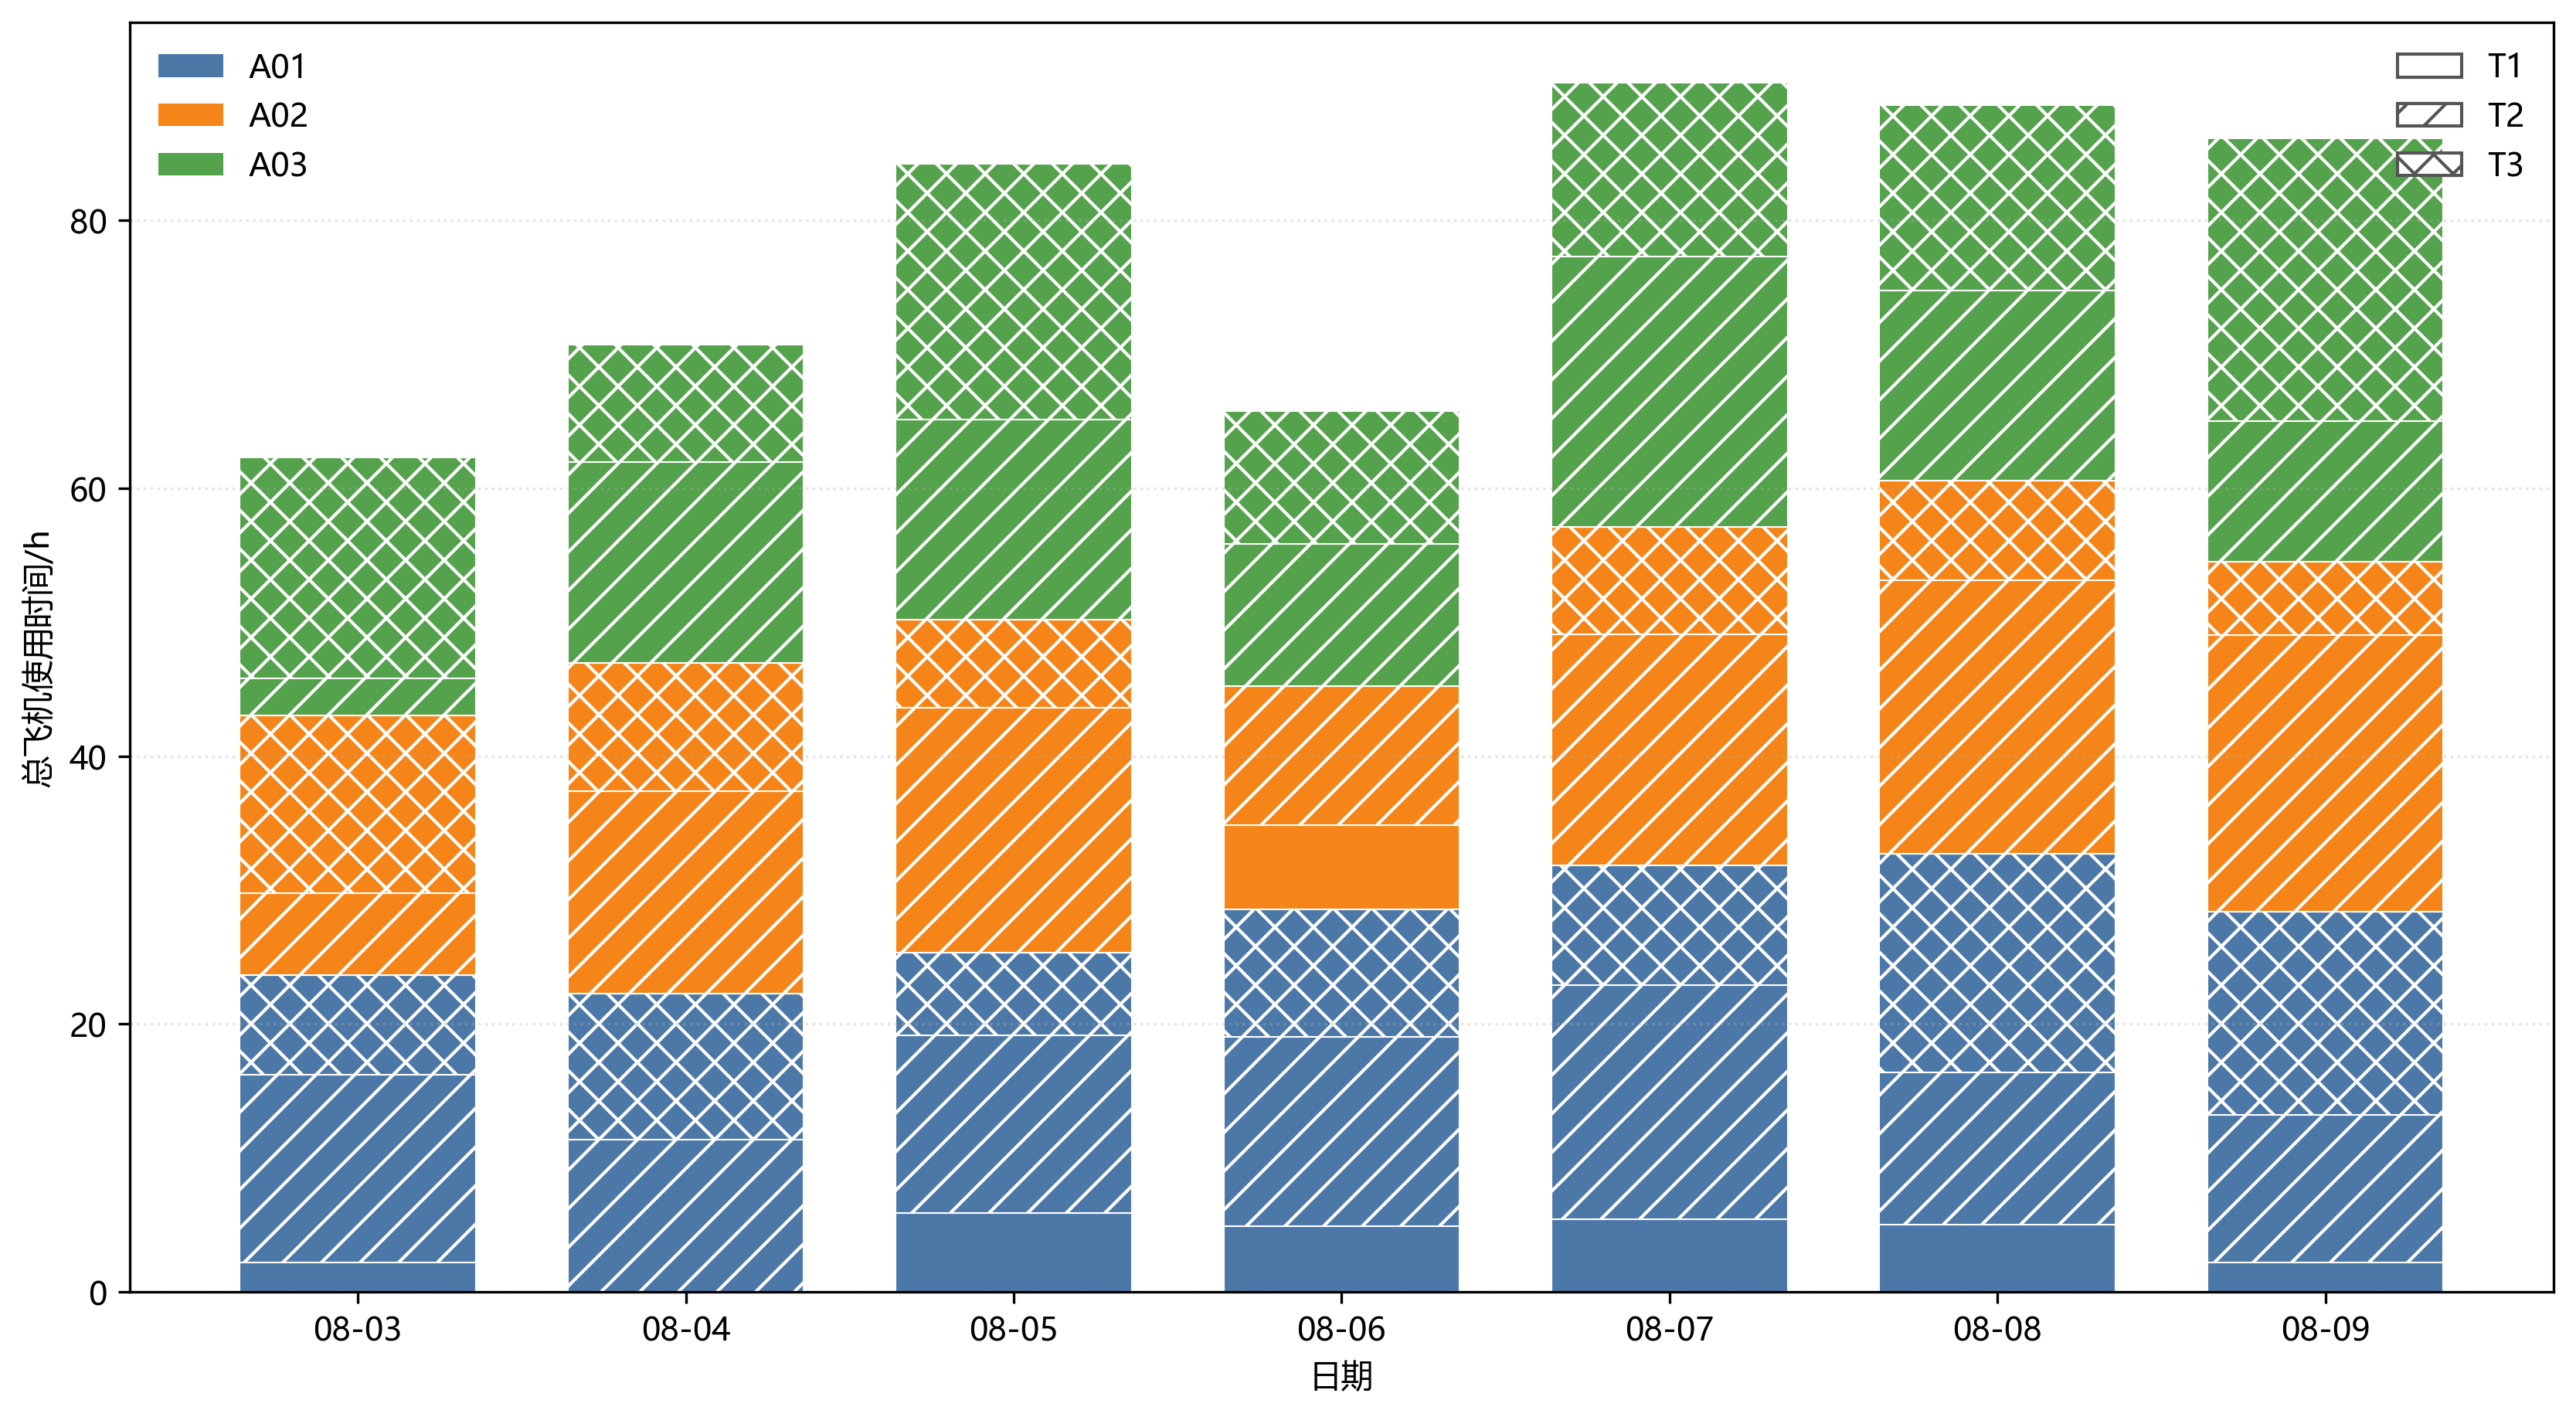
\includegraphics[width=0.92\textwidth]{outputs/figures/q3_daily_airport_workload.png}
\caption{各日期、机场和机型的飞机使用时间}
\label{fig:q3-workload}

\end{figure}

经过统计，本问题的164个架次中，随着海上着陆次数增加，单架次平均运输人数总体提高，但绕行和停靠增加使4至5次着陆架次的平均座位利用率有所下降。这体现了联合运输规模、动态上下客和航段利用效率之间的权衡。海上着陆次数和单架次座位利用率的总体分布如图~\ref{fig:q3-route-structure}所示。

% 架次结构表的解释之后紧接分布图

\begin{figure}[H]

\centering
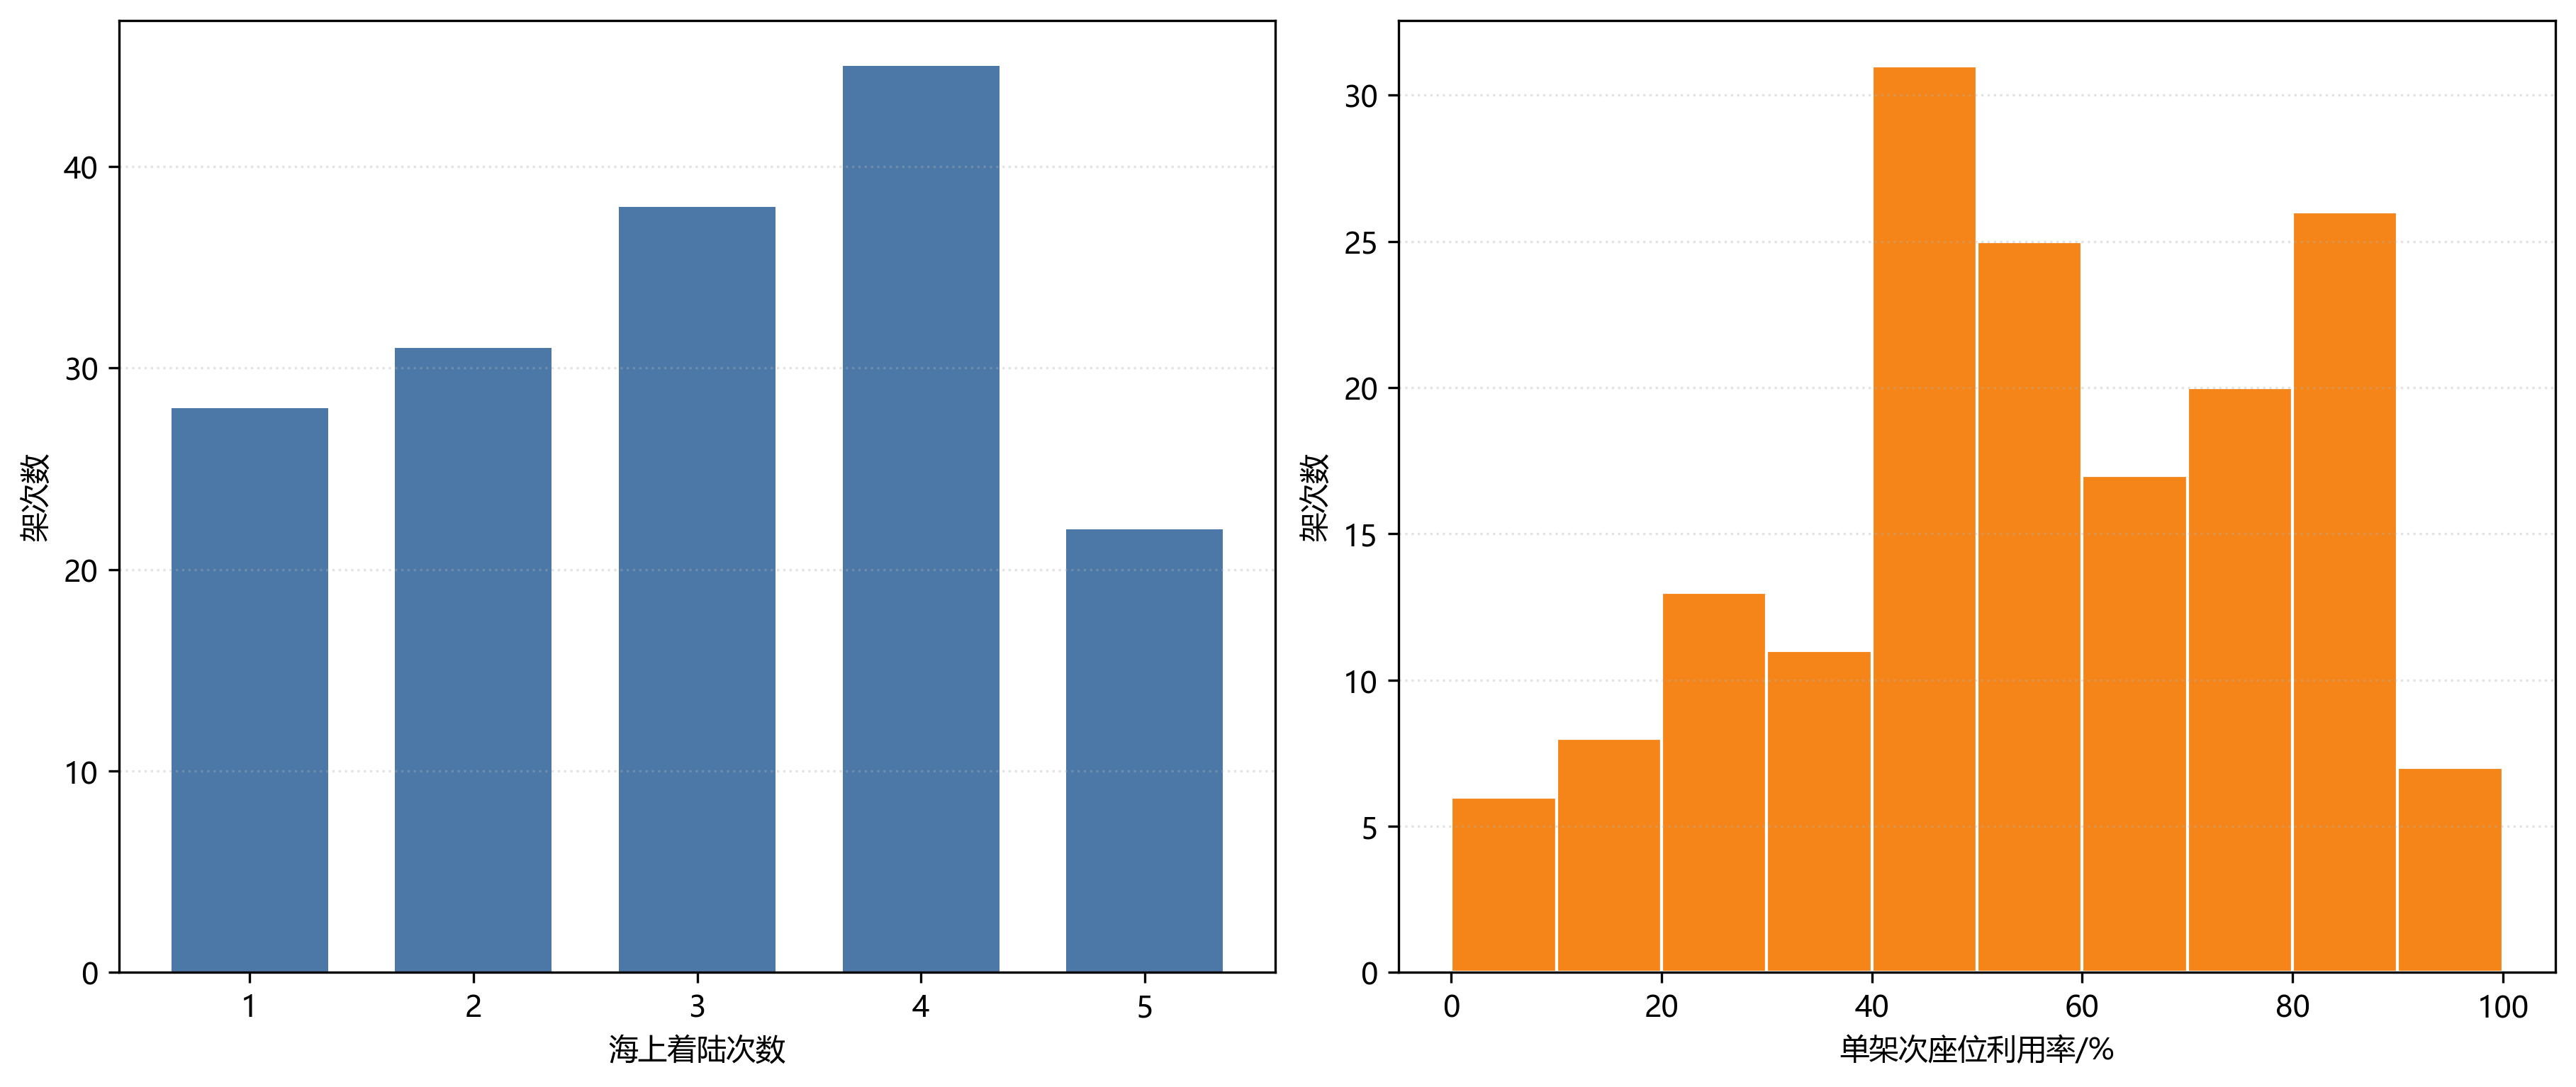
\includegraphics[width=0.92\textwidth]{outputs/figures/q3_route_structure.png}
\caption{海上着陆次数与单架次座位利用率分布}
\label{fig:q3-route-structure}

\end{figure}

不过由于我们在求解中的时空路线池由启发式邻域逐步生成，未枚举原问题的全部合法人员组合与运输路线，因此本文不能保证获得原始大规模问题的全局最优解，而将最终结果表述为限定搜索时间和当前生成路线池下，经独立校验得到的最佳已知可行方案。

%%%%%评价%%%%%
\section{模型评价}
\subsection{模型的优点}
\subsubsection{统一描述多类运输任务}
模型将出海、海返和设施间穿梭统一为带取送关系的单架次路径，并逐航段更新载客量和剩余燃油，能够处理重复停靠、先下后上和途中加油等情况。问题三进一步通过起飞时间区间和具体飞机的不重叠约束，落实人员时间窗、机场归属及30分钟周转要求。

\subsubsection{目标层次清晰，结果便于检验}
模型采用字典序优化，依次优化总飞机使用时间、人员总在途时间、燃油消耗和座位利用率，避免经验权重改变目标优先级。ALNS负责扩充候选路线，集合划分模型负责全局重组，降低了局部贪心造成次优解的可能。最终方案还通过独立回放检查人员覆盖、容量、燃油、时间窗和飞机占用，保证输出结果满足题目约束。

\subsection{模型的缺点}
\subsubsection{全局最优性受到路线池限制}
候选路线由启发式算法生成，未能枚举全部人员组合和停靠序列。因此，求解器返回的\texttt{OPTIMAL}仅表示当前路线池内达到最优，不能证明原问题的全局最优。本文所得结果应表述为限定计算时间和候选路线池下的最佳已知可行方案。

\subsubsection{结果对搜索参数具有一定依赖性}
邻域范围、路线池容量和计算时间分配均会影响求解结果。特别是问题三的基准时间$32887$分钟和154名临时人员均未完成全局最优性证明。后续可增加不同随机种子的重复实验，并分别检验$T\leq32886$和$Y\geq155$是否可行，以进一步评价解的稳定性和最优性差距。

%%%%%总结%%%%%
\section{总结}
本文针对海上油田人员运输问题，建立了由单架次可行性检查、候选路线生成和集合划分组成的优化模型。问题一完成1600名出海人员运输，共安排92个架次，总飞机使用时间为14991分钟；问题二联合安排4000名出海、海返及穿梭人员，共安排118个架次，总飞机使用时间为20751分钟。

问题三进一步考虑人员时间窗、24架具体飞机、机场运营时间和周转要求。第一阶段完成3840名非临时人员运输，得到32887分钟的最佳已知基准；第二阶段在不超过该基准的条件下完成154名临时人员运输，最终安排164个架次。独立回放表明，所得方案满足人员覆盖、容量、燃油、时间窗及飞机调度约束。由于候选路线空间未被完全枚举，本文结果属于有限计算条件下的最佳已知可行解，后续可通过构造下界和边界判定模型进一步加强最优性结论。

%%%%%参考文献%%%%%
\begin{thebibliography}{99}   % 99 是最大编号宽度

\end{thebibliography}

\section*{附录}
\appendix

\section{文件清单}

\noindent{支撑材料的文件列表清单：}
\begin{enumerate}
    \item 
    \item utils.py
\end{enumerate}

\section{代码}
\noindent{数据}
\lstinputlisting[language=Python]{}

\end{document}
